
%% Copyright 2009 Elsevier Ltd
%%
%% This file is part of the 'Elsarticle Bundle'.
%% ---------------------------------------------
%%
%% It may be distributed under the conditions of the LaTeX Project Public
%% License, either version 1.2 of this license or (at your option) any
%% later version.  The latest version of this license is in
%%    http://www.latex-project.org/lppl.txt
%% and version 1.2 or later is part of all distributions of LaTeX
%% version 1999/12/01 or later.
%%
%% The list of all files belonging to the 'Elsarticle Bundle' is
%% given in the file `manifest.txt'.
%%
%% Template article for Elsevier's document class `elsarticle'
%% with numbered style bibliographic references
%%
%% $Id: elsarticle-template-1a-num.tex 151 2009-10-08 05:18:25Z rishi $
%% $URL: http://lenova.river-valley.com/svn/elsbst/trunk/elsarticle-template-1a-num.tex $
%%
%%\documentclass[preprint,12pt]{elsarticle}

%% Use the option review to obtain double line spacing
\documentclass[preprint,review,12pt]{elsarticle}

%% Use the options 1p,twocolumn; 3p; 3p,twocolumn; 5p; or 5p,twocolumn
%% for a journal layout:
%% \documentclass[final,1p,times]{elsarticle}
%% \documentclass[final,1p,times,twocolumn]{elsarticle}
%% \documentclass[final,3p,times]{elsarticle}
%% \documentclass[final,3p,times,twocolumn]{elsarticle}
%% \documentclass[final,5p,times]{elsarticle}
%% \documentclass[final,5p,times,twocolumn]{elsarticle}

%% if you use PostScript figures in your article
%% use the graphics package for simple commands
%% \usepackage{graphics}
%% or use the graphicx package for more complicated commands
%% \usepackage{graphicx}
%% or use the epsfig package if you prefer to use the old commands
%% \usepackage{epsfig}

%% The amssymb package provides various useful mathematical symbols
\usepackage{amssymb}
\usepackage{amsfonts}
\usepackage{amsmath}
\usepackage{pdflscape}
\usepackage{graphicx}
\graphicspath{{figures/}}
\usepackage[figuresright]{rotating}
\usepackage{bbm,bm}
\usepackage{subfigure}
\usepackage{color}
\usepackage{topcapt}
\usepackage{multirow} % multi row for table
\usepackage{ulem} %% using delete symbol
\newcommand{\ud}{\textrm{d}}

%% The amsthm package provides extended theorem environments
%% \usepackage{amsthm}

%% The lineno packages adds line numbers. Start line numbering with
%% \begin{linenumbers}, end it with \end{linenumbers}. Or switch it on
%% for the whole article with \linenumbers after \end{frontmatter}.
%% \usepackage{lineno}

%% natbib.sty is loaded by default. However, natbib options can be
%% provided with \biboptions{...} command. Following options are
%% valid:

%%   round  -  round parentheses are used (default)
%%   square -  square brackets are used   [option]
%%   curly  -  curly braces are used      {option}
%%   angle  -  angle brackets are used    <option>
%%   semicolon  -  multiple citations separated by semi-colon
%%   colon  - same as semicolon, an earlier confusion
%%   comma  -  separated by comma
%%   numbers-  selects numerical citations
%%   super  -  numerical citations as superscripts
%%   sort   -  sorts multiple citations according to order in ref. list
%%   sort&compress   -  like sort, but also compresses numerical citations
%%   compress - compresses without sorting
%%
%% \biboptions{comma,round}

% \biboptions{}


\journal{Computers and Geotechnics}

\begin{document}

\begin{frontmatter}

%% Title, authors and addresses

%% use the tnoteref command within \title for footnotes;
%% use the tnotetext command for the associated footnote;
%% use the fnref command within \author or \address for footnotes;
%% use the fntext command for the associated footnote;
%% use the corref command within \author for corresponding author footnotes;
%% use the cortext command for the associated footnote;
%% use the ead command for the email address,
%% and the form \ead[url] for the home page:
%%
%% \title{Title\tnoteref{label1}}
%% \tnotetext[label1]{}
%% \author{Name\corref{cor1}\fnref{label2}}
%% \ead{email address}
%% \ead[url]{home page}
%% \fntext[label2]{}
%% \cortext[cor1]{}
%% \address{Address\fnref{label3}}
%% \fntext[label3]{}

\title{Forms of energy dissipated in the damaged zone of of underground cavities: Theoretical analysis and Finite Element Modeling}

%% use optional labels to link authors explicitly to addresses:
%% \author[label1,label2]{<author name>}
%% \address[label1]{<address>}
%% \address[label2]{<address>}

\author{Hao Xu, Chlo\'e Arson}

\address{School of Civil and Environmental Engineering,
Georgia Institute of Technology, Atlanta, Georgia 30332, U.S.A.}

\begin{abstract}
%% Text of abstract


\end{abstract}

\begin{keyword}
%% keywords here, in the form: keyword \sep keyword
Damage model \sep anisotropic \sep deviatoric stress \sep stress path
\sep thermodynamic framework
%% MSC codes here, in the form: \MSC code \sep code
%% or \MSC[2008] code \sep code (2000 is the default)

e\end{keyword}

\end{frontmatter}

%%
%% Start line numbering here if you want
%%
% \linenumbers

%% main text

\section{Introduction}

%==========================================================================================
\section{SoA on model of damage inducing irreversible deformation}

\subsection{damage and plasticity} 
The first work relating plasticity to damage is introduced by Lubliner \cite{Lubliner1989} in concrete damage model, which defined the damage variable as the ratio of the dissipated plastic energy. In order to ensure the positivity of the damage variable within the 
framework of the Continuum Damage Mechanics, the damage potential is always
proposed as the homogeneous function in terms of damage driving force. Due 
to the different constrains for the evolution of damage and irreversible 
strain, in general, the damage potential and the inelastic strain potential
are chosen differently, which means the non-associated flow rule is used in
the model. The plasticity theory is coupled  to a damage model 
to reflect the plastic (irreversible) deformation upon unloading \cite{Abualrub2010,Cicekli2007,Murakami1996}.      
$\mathbb{C}(\bm\Omega)+\epsilon^{p}$

\subsection{extended CDM}
Instead of coupling with the plasticity for permanent strain, the residual strain representing the crack opening after unloading can be taken into account by proposing a damage potential. 
\cite{Halm1998,Homand-Etienne1998}
Enriching the framework of CDM with microscopic properties of geomaterials is another strategy to account for the inelastic strain $\mathbb{C}(\bm\Omega)+\epsilon^{id}$

\subsection{Multiscale strategy}
 
The relationship between fracture mechanics and damage mechanics based on the thermodynamic considerations is built by Mazars \& Pijaudier-Cabot \cite{Mazars1996}. This lead to the equivalent crack concept, in passing from a continuous damage zone to a discrete fracture. Distinct energy terms for the fundamental of cohesive method are studied by Gurtin, and he derived the energy release rate for a sharp crack surrounding by a homogeneous hyperelastic body.
 
\subsection{presentation of extended CDM approach (put equations of the model in appendix)}

\subsection{thermodynamic consistency} 

%=====================================================================================
\section{Outline of the DSID model}
\subsection{theoretical framework and algorithms} 
\begin{figure}[htbp]
\begin{center}
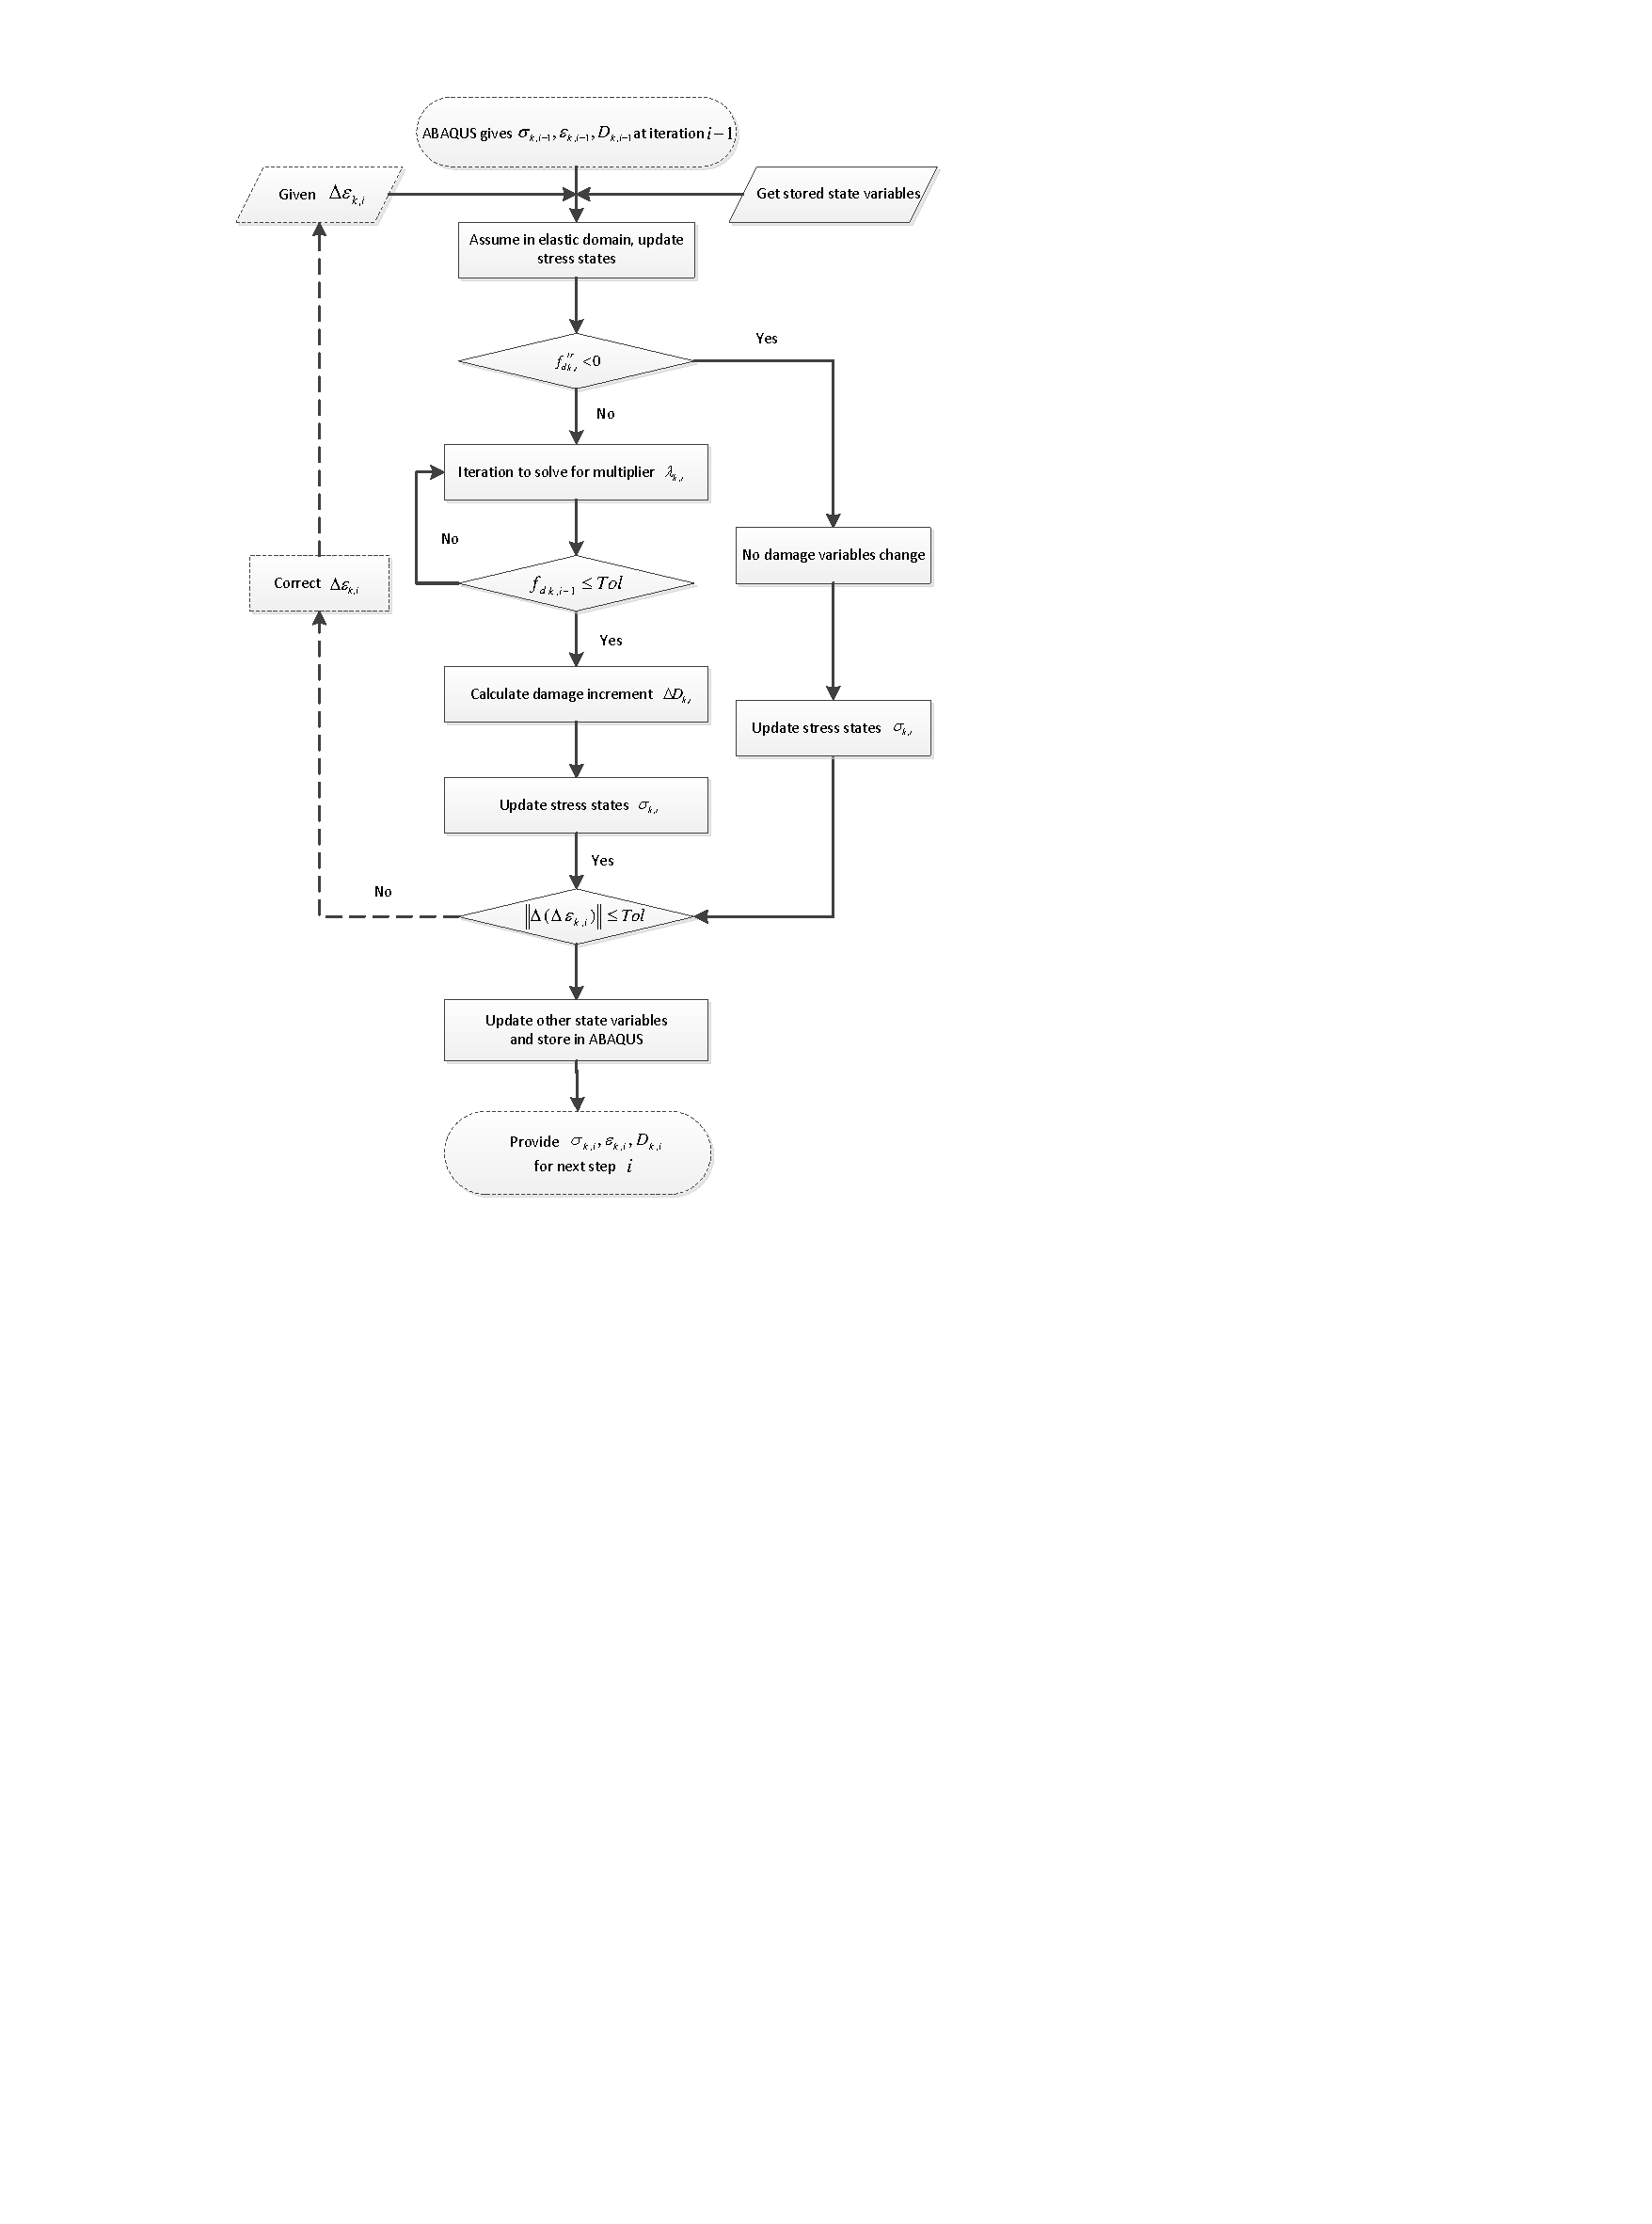
\includegraphics[width=\textwidth]{flowchart2.pdf}
\caption{DSID model}
\label{fig:energy}
\end{center}
\end{figure}
\subsection{Numerical implementation (MATLAB, ABAQUS, residual)}
%=====================================================================================
\section{Element Level: analysis of the forms of energy dissipation}
\subsection{Micro-scopic effects -- Energy dissipation}
%
The Inequality of Clausisus-Duhem is derived from the combination of the two first laws of thermodynamics:
%
\begin{equation}
 \label{eq:ICD1}
  \dot\varPhi_s=\bm\sigma:\dot{\bm\varepsilon}-\dot{\psi}_s \ge 0
\end{equation}
%
The free energy rate writes:
%
\begin{equation}
\label{eq:ratefreeenergy}
    \dot{\psi}_s=\frac{\partial \psi_s}{\partial \bm\varepsilon^E}:\dot{\bm\varepsilon}^E
    + \frac{\partial \psi_s}{\partial \bm\varOmega}:\dot{\bm\varOmega}
\end{equation}
%
The dissipation potential of solid skeleton should satisfy the Clausis-Duhem Inequality:
%
\begin{equation}\label{ICD2}
   \dot\varPhi_s=\bm\sigma:\dot{\bm\varepsilon}^{id}+\bm{Y}:\dot{\bm\varOmega} \ge 0
\end{equation}
%
The work by the external force is $\bm\sigma:\dot{\bm\varepsilon}$ in each step, and $\dot\varPhi_s$ is the dissipated energy during each load increment. The strain energy stored in the solid body is $\frac{1}{2}\bm\sigma:\bm\varepsilon^E$. The energy lost in the loading should be always non-negative.
%
%\begin{figure}[htbp]
%\begin{center}
%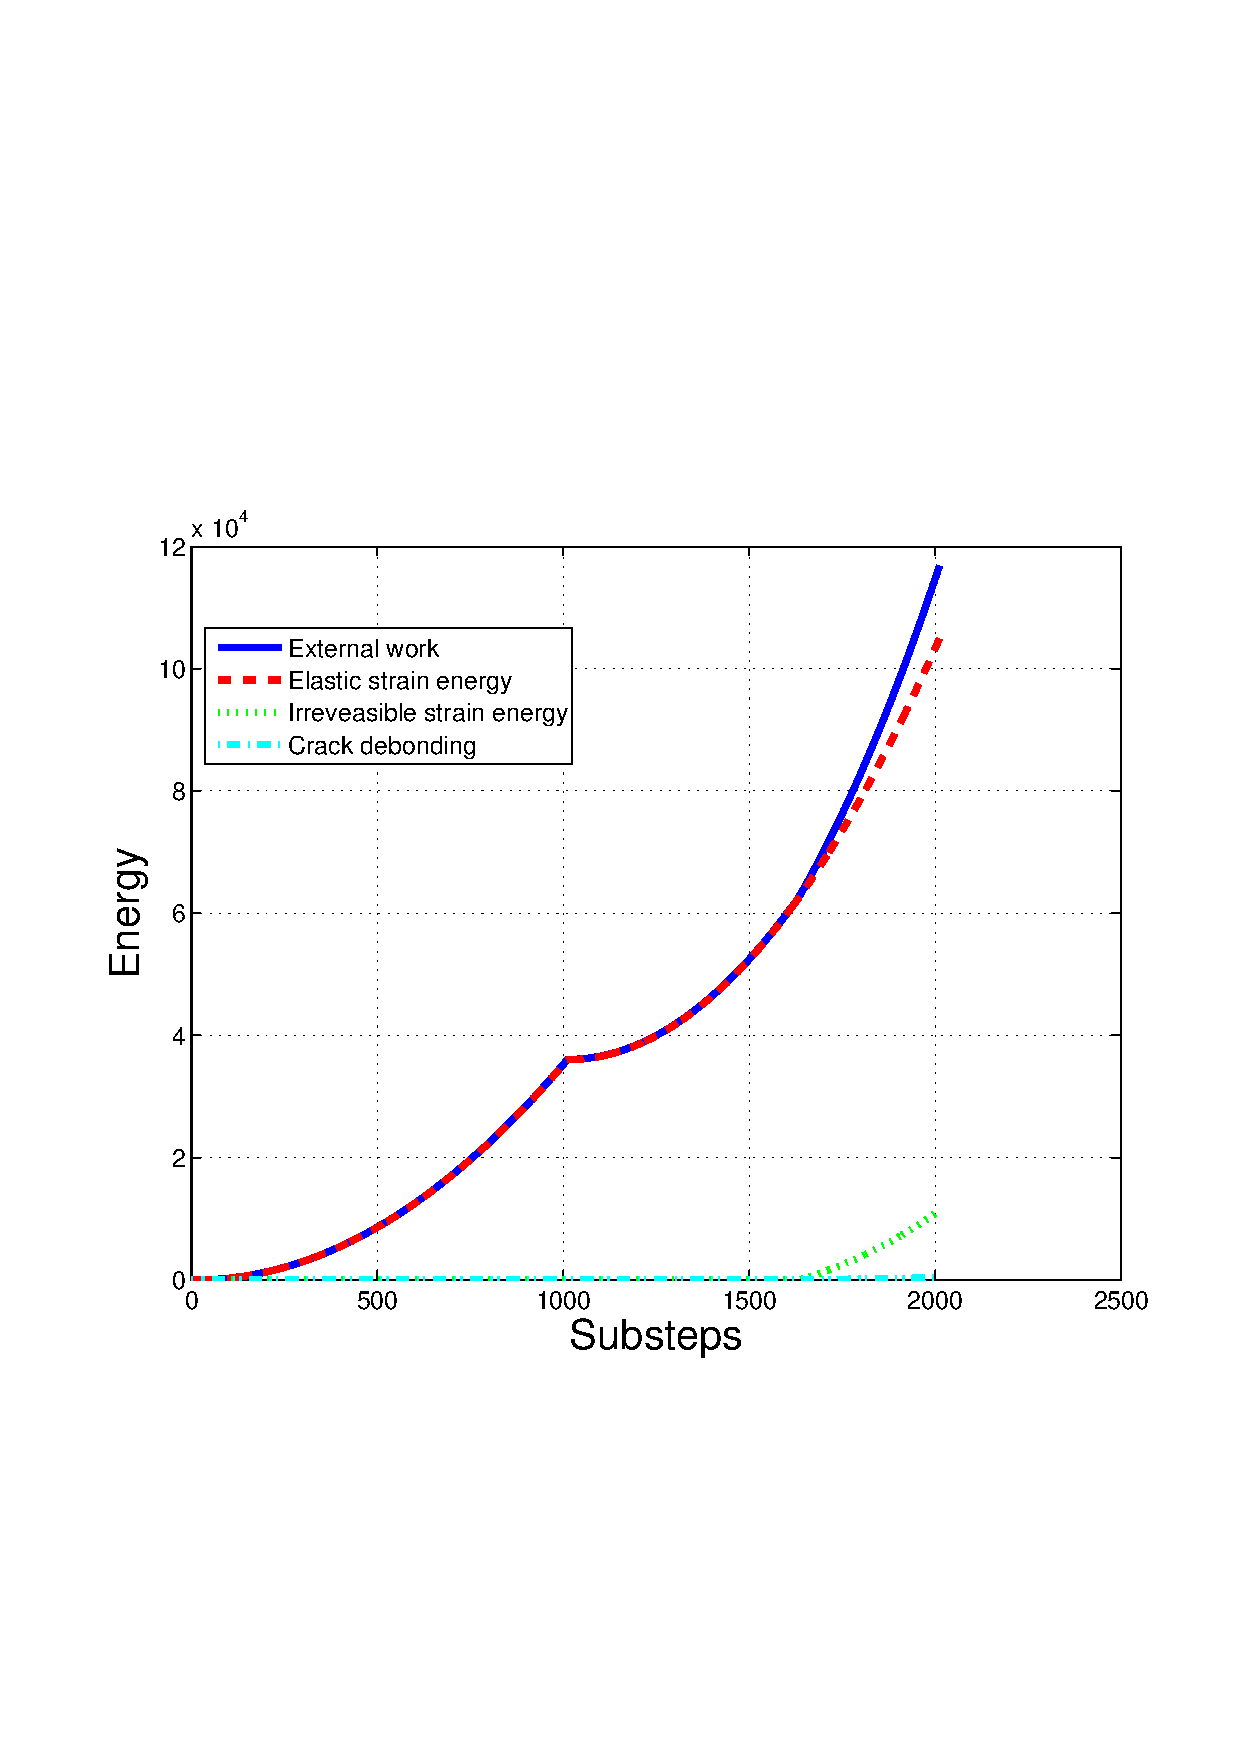
\includegraphics[width=\textwidth]{energy.png}
%\caption{Energy costume during loading}
%\label{fig:energy}
%\end{center}
%\end{figure}
%
\begin{equation}\label{eq:ICD3}
   \bm\sigma:\dot{\bm\varepsilon}^{id}+\bm{Y}:\dot{\bm\varOmega} \ge 0
\end{equation}
%---------------------------------------------------------------------
\subsubsection{Types of energy dissipation}
%---------------------------------------------------------------------
The work by the external force is $\bm\sigma:\dot{\bm\varepsilon}$ in each step, so the accumulate work is $\int \bm\sigma:\dot{\bm\varepsilon} \,\ud t$. The accumulate strain energy stored in the solid body is $\frac{1}{2}\bm\sigma:\bm\varepsilon^E$, and the dissipated energy is the differential between the the differential between external work and recoverable strain energy. The mechanical energy lost, $\int \dot\varPhi_d \, \ud t$, in the loading is the area displayed in figure \ref{fig:energylost} with pink color and should be always non-negative, while the recoverable elastic strain energy is the area of the triangle as figure \ref{fig:energylost} with light green color.
%
\begin{equation}
   \label{eq:elost}
   \int \dot\varPhi_{d} \, \ud t = \int\bm\sigma:\dot{\bm\varepsilon}\,\ud t -\frac{1}{2}\bm\sigma:\bm\varepsilon^E\ge 0
\end{equation}
%
\begin{figure}[htbp]
   \centering
  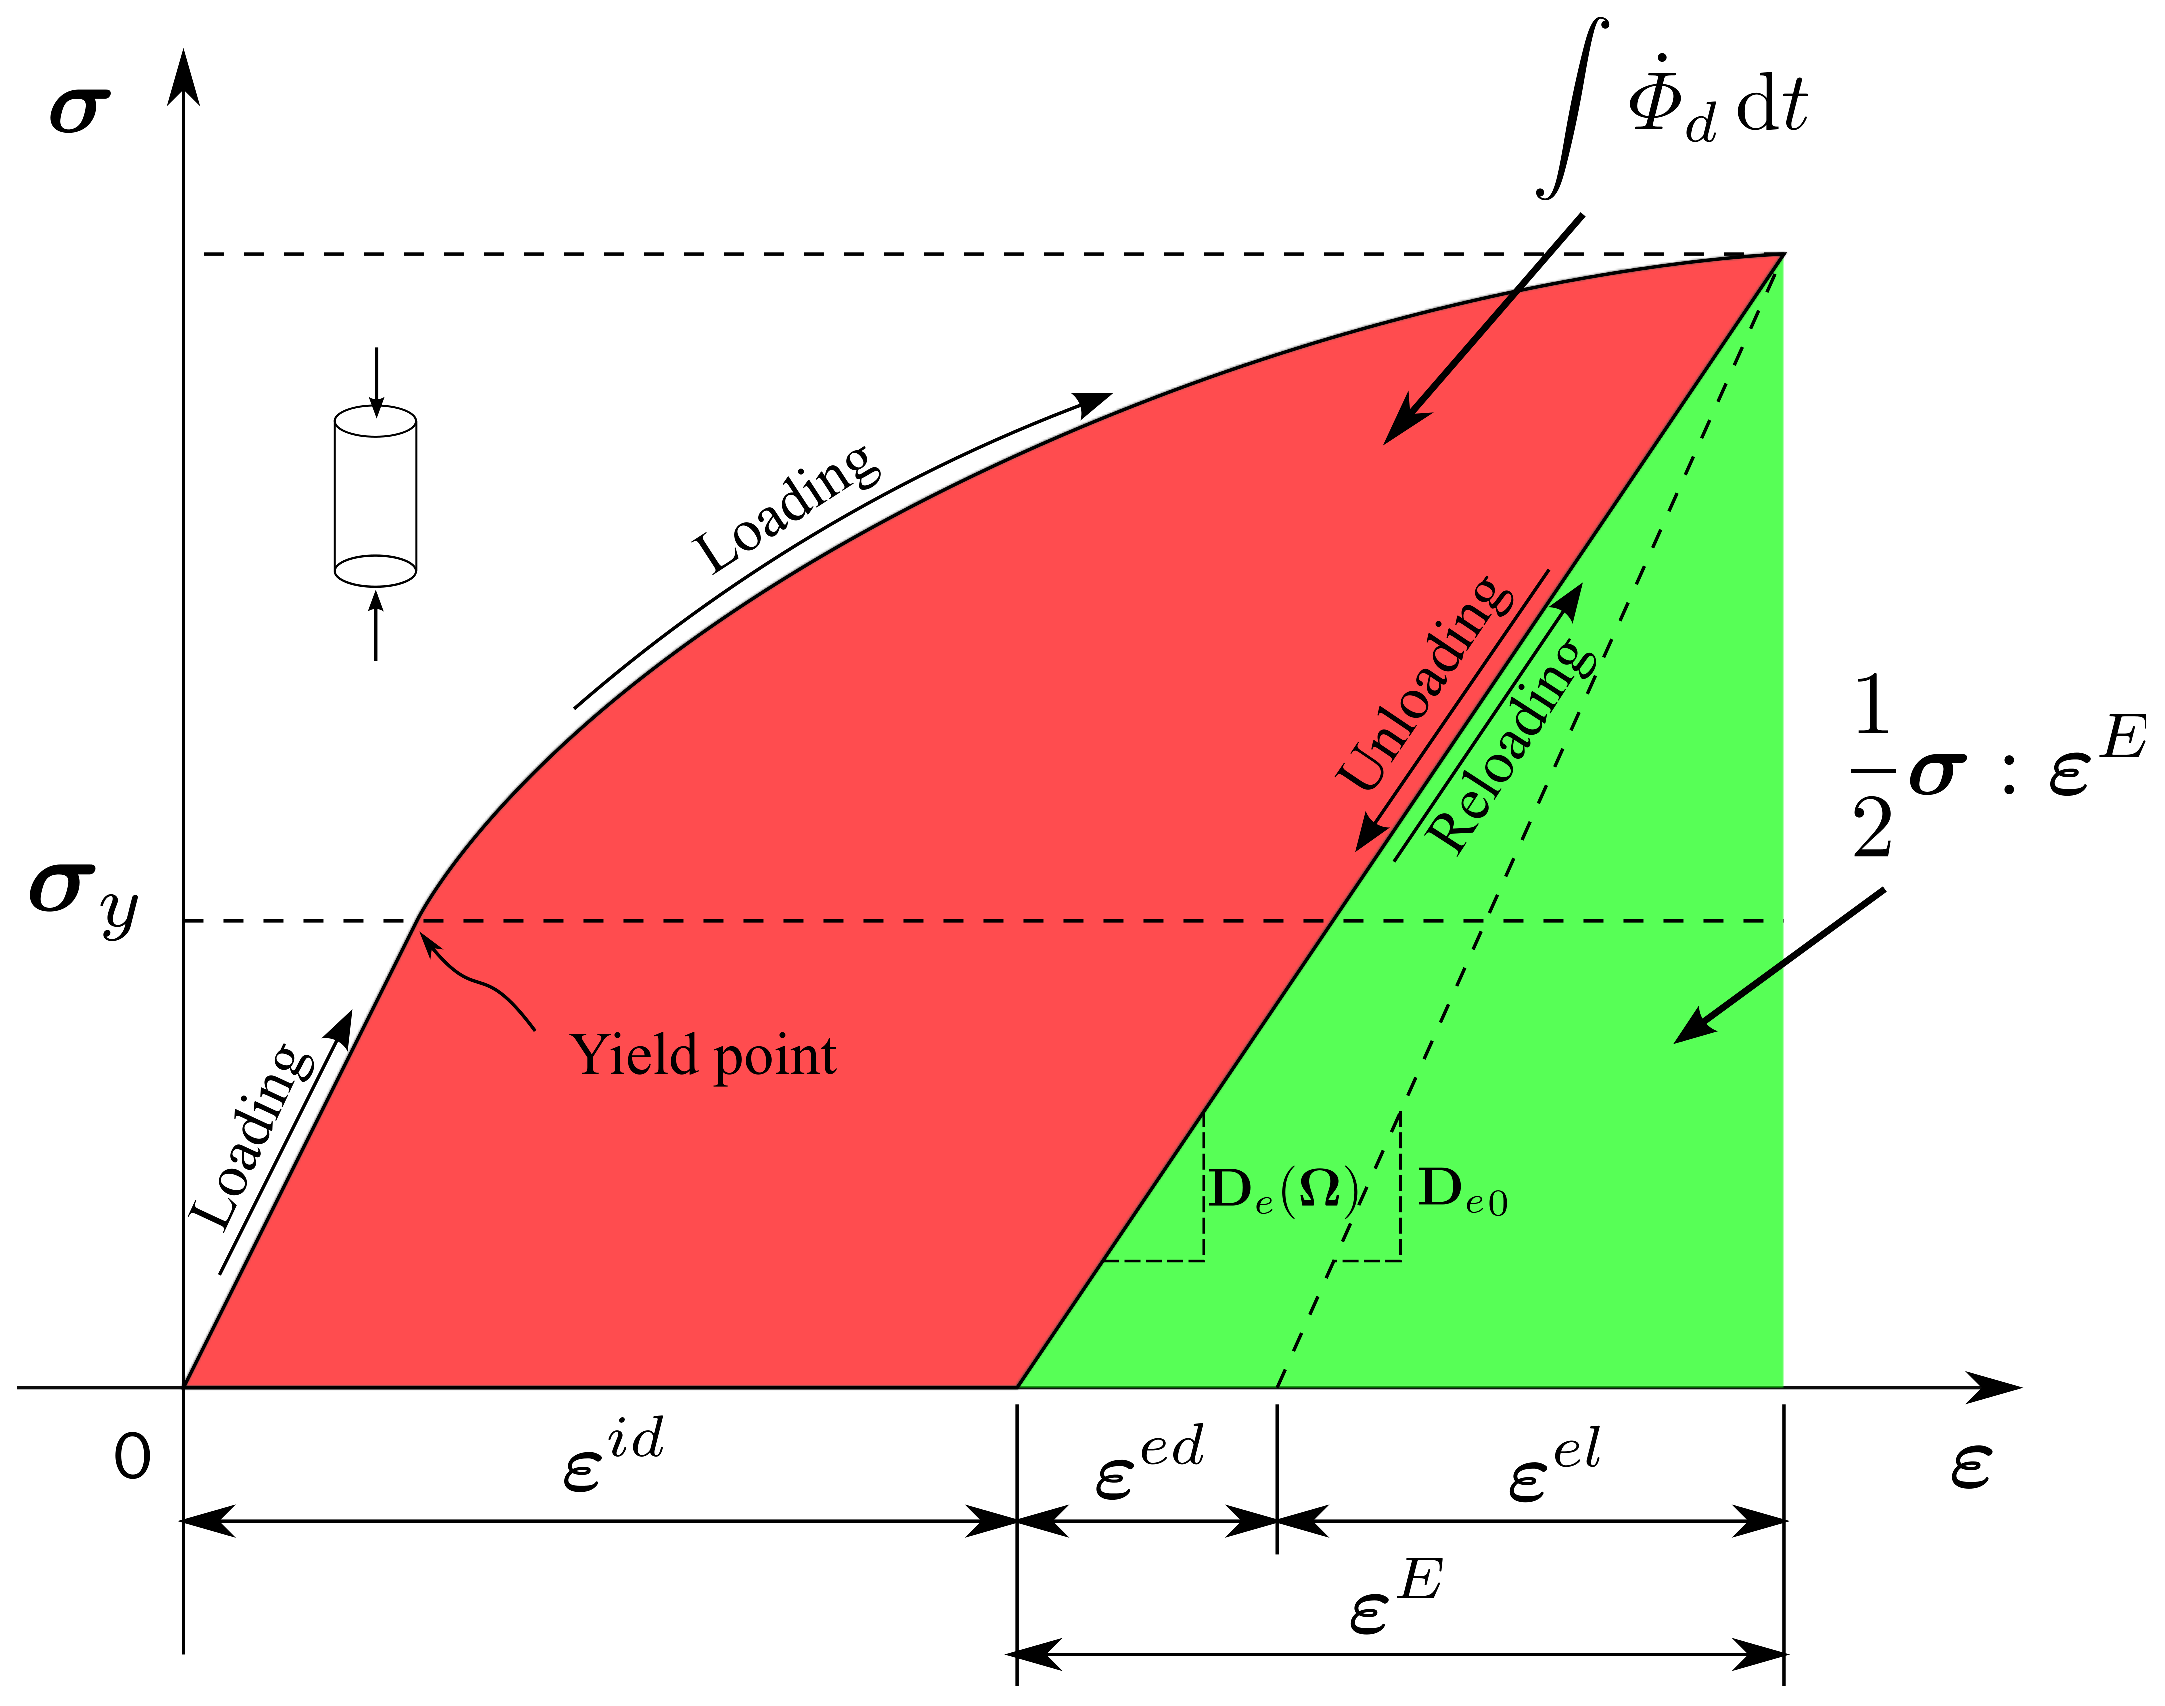
\includegraphics[width=0.6\textwidth]{inkscape/energy_lost/energy_lost2.eps}
   \caption{Energy spent in one loading process}
   \label{fig:energylost}
\end{figure}
\
\\
The energy dissipated by damage is concluded into two means, crack generating without additional deformation and debonding paris of crack surfaces. Both of these two approaches can be represented by the mechanical response. Crack generation decrease the stiffness of material, which can increase the capacity that material stores the energy; while debonding is related to non-linear strains. Since there are no other ways of energy transfer (thermal transport or radiation), the energy should be conserved in total. Based on response of material, all of the work by external loading should be splitted into three parts as figure \ref{fig:energysplit1} shows (The white part of energy is compensated by the extra part of the energy, related to irreversible strain, above the stress curve). It is also true from the strain decomposition in another side. The energy conservation is expressed as:
%
\begin{equation}
  \label{eq:econserv}
   \int\bm\sigma:\dot{\bm\varepsilon}\,\ud t = \int\bm\sigma:\dot{\bm\varepsilon}^{el}\,\ud t +
   \int\bm\sigma:\dot{\bm\varepsilon}^{ed}\,\ud t + \int\bm\sigma:\dot{\bm\varepsilon}^{id}\,\ud t
\end{equation}
%
\begin{figure}[htbp]
   \centering
   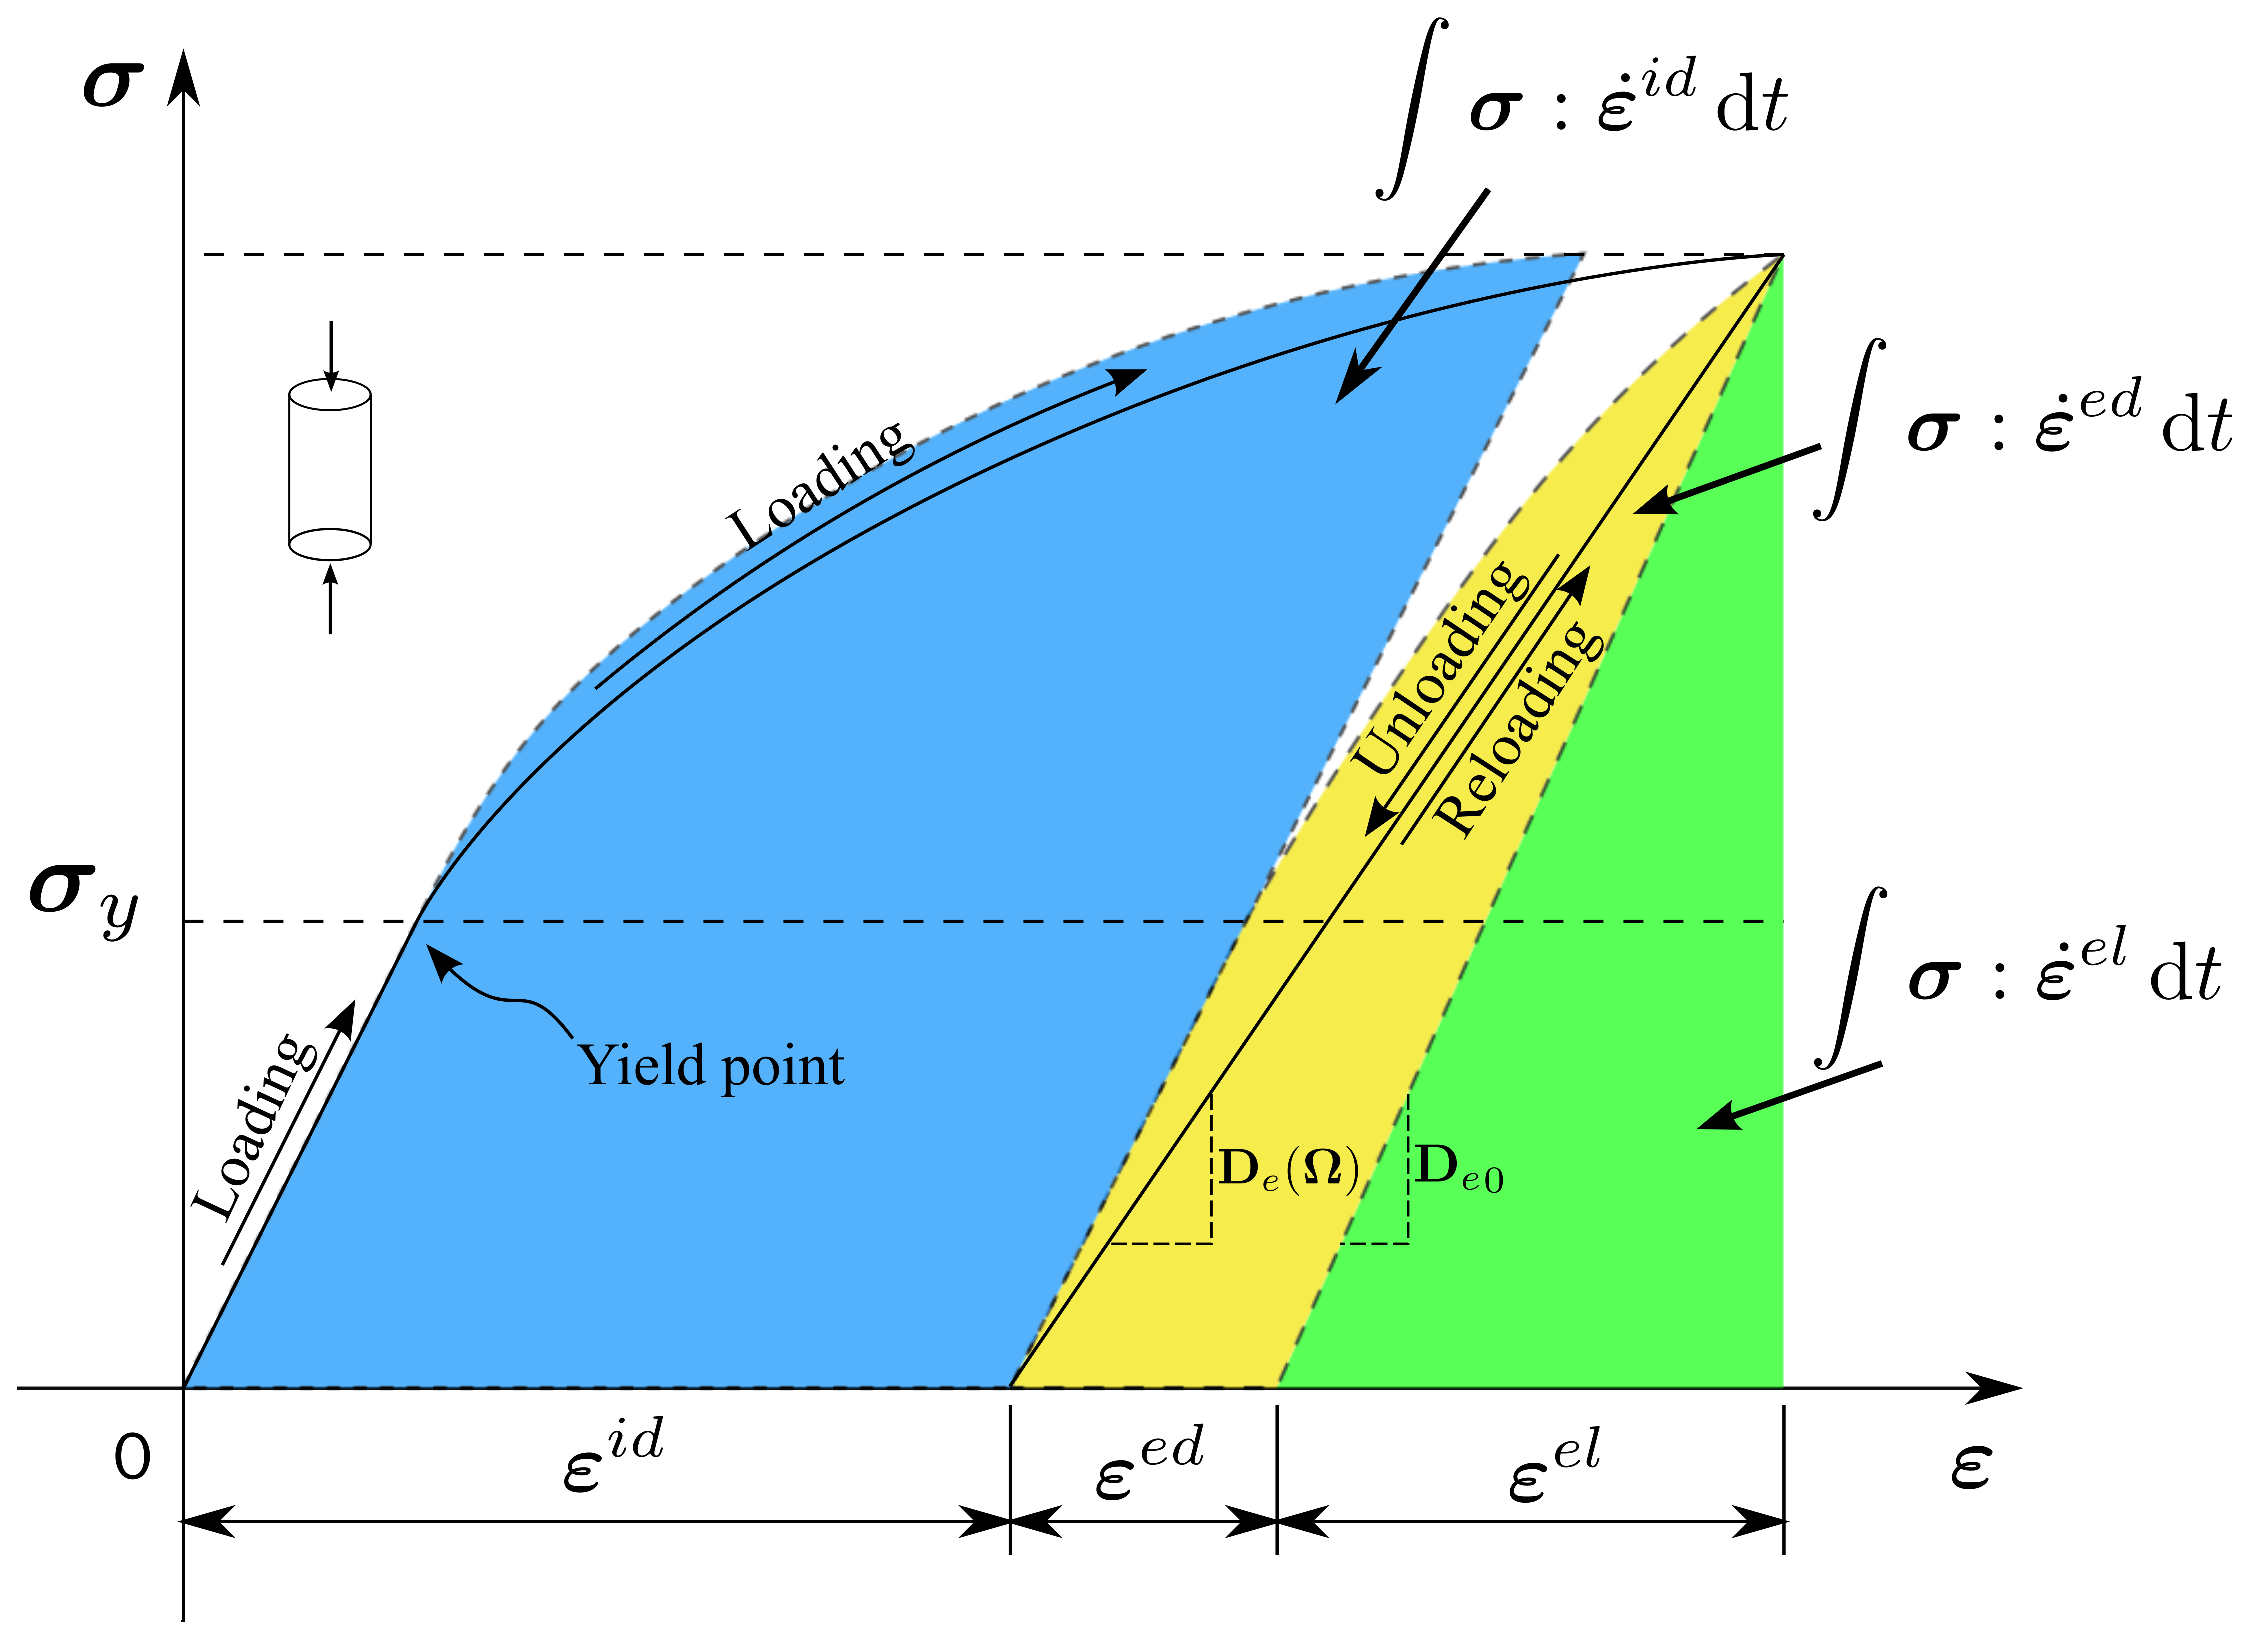
\includegraphics[width=0.6\textwidth]{inkscape/energy_split/energy_split.eps}
   \caption{Energy splitting in one loading process}
   \label{fig:energysplit1}
\end{figure}
\
\\
There are two parts of the energy related to elasto-damage strain, $\bm\varepsilon^{ed}$. Not both of the elasto-damage strain is dissipated, some of them is stored in the solid body as strain energy ($\frac{1}{2}\bm\sigma:\dot{\bm\varepsilon}^{ed}$); the other is dissipated (if material is unloaded), which won't induce the any strain increment. This part noted as $\int \bm{Y}:\dot{\bm\varOmega}\,\ud t$ is due to the crack generating but no displacement (figure \ref{fig:energysplit2}).
%
\begin{equation}\label{eq:esplit1}
   \int\bm\sigma:\dot{\bm\varepsilon}^{ed}\,\ud t = \frac{1}{2}\bm\sigma:\bm\varepsilon^{ed} +
   \int\bm{Y}:\dot{\bm\varOmega}\,\ud t
\end{equation}
%
The energy related to debonding of the crack surfaces will be dissipated ($\int \bm\sigma:\dot{\bm\varepsilon}^{id}\,\ud t$ related to irreversible strain) or stored ($\frac{1}{2}\bm\sigma:\dot{\bm\varepsilon}^{ed}$, one part of energy related to elasto-damage strain.)

\begin{figure}[htbp]
   \centering
   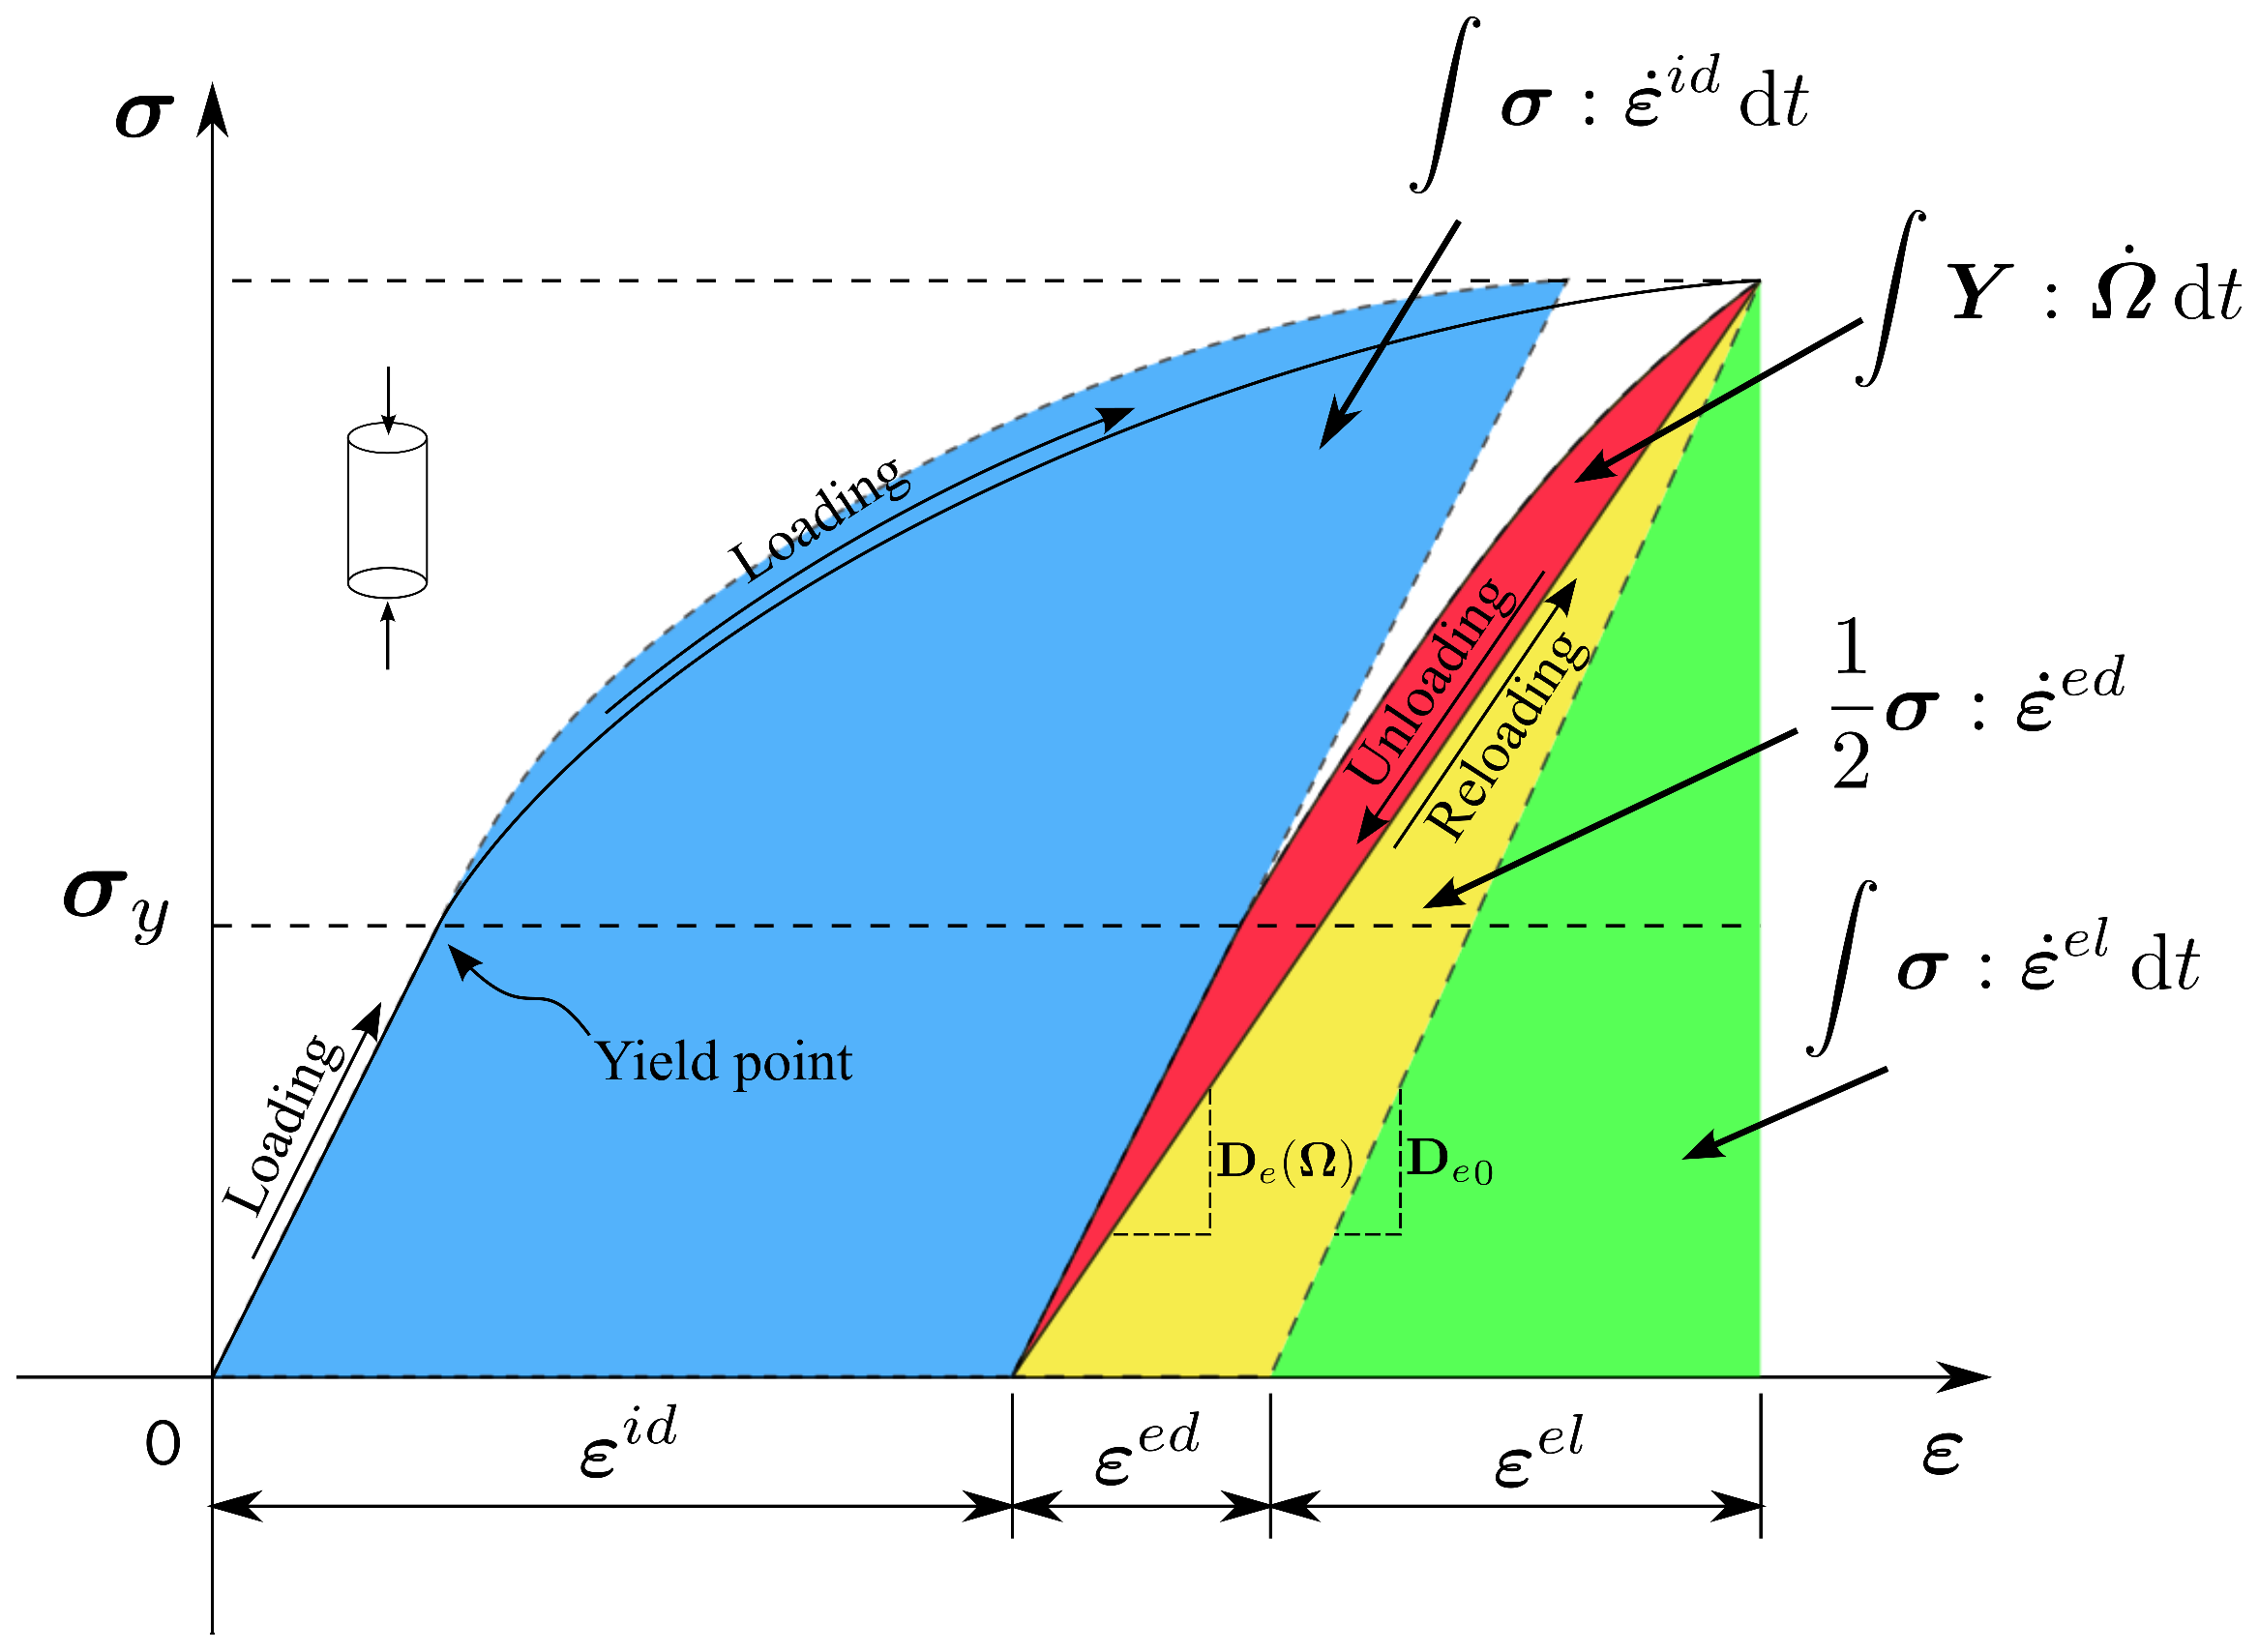
\includegraphics[width=0.6\textwidth]{inkscape/energy_split/energy_split2.eps}
   \caption{Energy splitting in one loading process}
   \label{fig:energysplit2}
\end{figure}
\
\\
Based on the mechanical part, the lost of the energy is dissipated by the irreversible strain and crack generation due to damage.
%
\begin{equation}\label{eq:elost2}
   \int \dot\varPhi_{d} \, \ud t = \int\bm\sigma:\dot{\bm\varepsilon}^{id}\,\textrm{d}t + \int \bm{Y}:\dot{\bm\varOmega}\,\ud t \ge 0
\end{equation}
%
Therefore, the following equation is hold:
%
\begin{equation}
   \label{eq:energy2}
   \int \bm\sigma:\dot{\bm\varepsilon}\,\ud t -\frac{1}{2}\bm\sigma:\bm\varepsilon^E = \int \bm\sigma:\dot{\bm\varepsilon}^{id}\,\ud t+\int \bm{Y}:\dot{\bm\varOmega}\,\ud t
\end{equation}
%
If in the FEM, it could be written in the summation of all increments.
%
\begin{equation}
   \label{eq:energyFEM1}
   \sum \bm\sigma_{\theta n}:\dot{\bm\varepsilon}_n -\frac{1}{2}\bm\sigma_n:\bm\varepsilon^E_{n} = \sum \bm\sigma_{\theta n}:\dot{\bm\varepsilon}^{id}_n+\sum \bm{Y}_{\theta n}:\dot{\bm\varOmega}_{n}
\end{equation}
Where $\bm\sigma_{\theta n}$ and $\bm{Y}_{\theta n}$ are the resultant stress and damage force during each increment when calculating the energy change:
\begin{align}
    \bm\sigma_{\theta n} = & \ (1-\theta)\bm\sigma_{n-1} + \theta \, \bm\sigma_{n} \\
    \bm{Y}_{\theta n} = & \ (1-\theta)\bm{Y}_{n-1} + \theta \, \bm{Y}_{n}
\end{align}
$\theta$ is the approximation factor.
The total elastic strain can be decomposed into:
\begin{equation}
   \label{eq:energy}
   \bm\varepsilon^E_{n} = \bm\varepsilon^E_{n-1} + \dot{\bm\varepsilon}^E_{n} = \bm\varepsilon^E_{n-1} + \dot{\bm\varepsilon}_{n} - \dot{\bm\varepsilon}^{id}_{n}
\end{equation}
%The equation \ref{eq:energyFEM1} is reorganized as:
%\begin{equation}
%   \label{eq:energyFEM2}
%      \begin{split}
%   & \left( \bm\sigma_{\theta n} - \frac{1}{2}\bm\sigma_n\right):\dot{\bm\varepsilon}^{id}_{n} + \bm{Y}_{\theta n}:\dot{\bm\varOmega}_{n}
%   \\
%   = & \sum\bm\sigma_{\theta n}:\dot{\bm\varepsilon}_n-\frac{1}{2}\bm\sigma_n:(\bm\varepsilon^{E}_{n-1}+\dot{\bm\varepsilon}_n) - \sum\bm\sigma_{\theta n-1}:\dot{\bm\varepsilon}^{id}_{n-1}-\sum \bm{Y}_{\theta n-1}:\dot{\bm\varOmega}_{n-1}
%   \end{split}
%\end{equation}
%--------------------------------------------------------------------------------------------
\subsection{Limitations of the DSID Model}
%
\begin{enumerate}
\item Meso-scopic effects
\
\\
The ``splitting effects'' and ``crossing effects'' are considered in the DSID model. Both of them follow the Griffth criterion for the mode I failure in rocks. Therefore, the damage generated by pure shear stress and the damage induced by the equivalent principal stress are equal. The equivalence of these two status is lack of the microscopic effects to account for the difference between shear failure and tensile failure. 
%
\item Micro-scopic effects
\
\\
Indeedly, the DSID model does not include the failure mechanisms in micro-scale, but the crack debonding is captured by the damage model in terms of the energy. The splitting of the crack surfaces is the micro-scopic effect 
\end{enumerate}

%%%%%%%%%%%%%%%%%%%%%%%%%%%%%%%%%%%%%%%%%%%%%%%%%%%%%%%
\subsection{Numerical Simulations of energy dissipation at element level}

a few cases for 1 2 3, maps showing $\Phi$ dissipated $W_e$ $W_{ed}$

$E$, $\nu$ (granite, shale, salt rock and claystone)

parametric study on the state of the rock (instead of stress)

%--------------------------------------------------------------------------------------------
\paragraph{Energy dissipation on different types of stress paths}
\
\\
\begin{enumerate}
\item Uniaxial Tensile test
\
\\
A uniaxial tensile test is computed with a 100 MPa pure shear stress in the REV.
\
\\
\begin{figure}[htbp]
\subfigure[Types of Energy]{
\label{fig:TypesOfEnegyTen}
\begin{minipage}[b]{0.48\textwidth}
\centering
\vspace{-3cm}
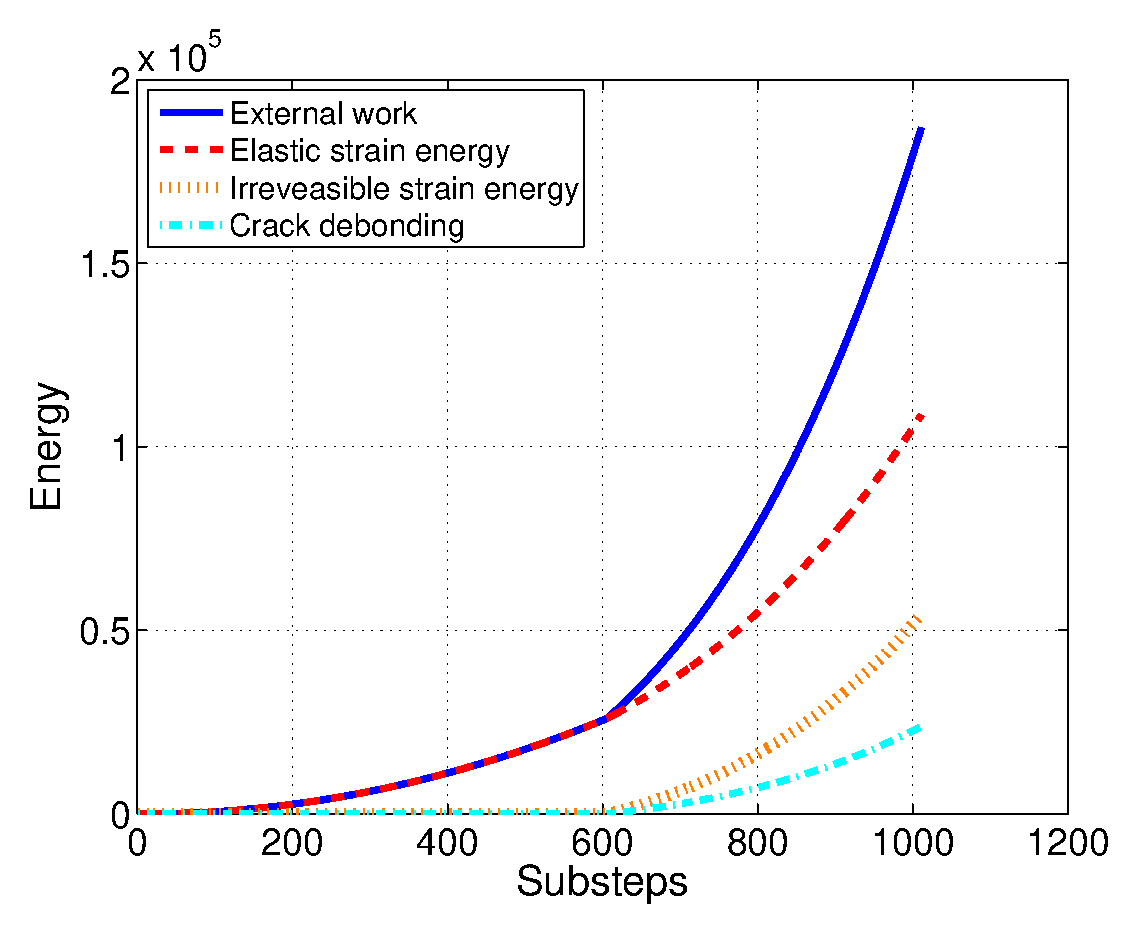
\includegraphics[width=\textwidth]{MRC/simple/tensile/energy1.eps}
\end{minipage}}
\subfigure[Percentages of Each Energy]{
\label{fig:PercentagesOfEachEnergy}
\begin{minipage}[b]{0.48\textwidth}
\centering
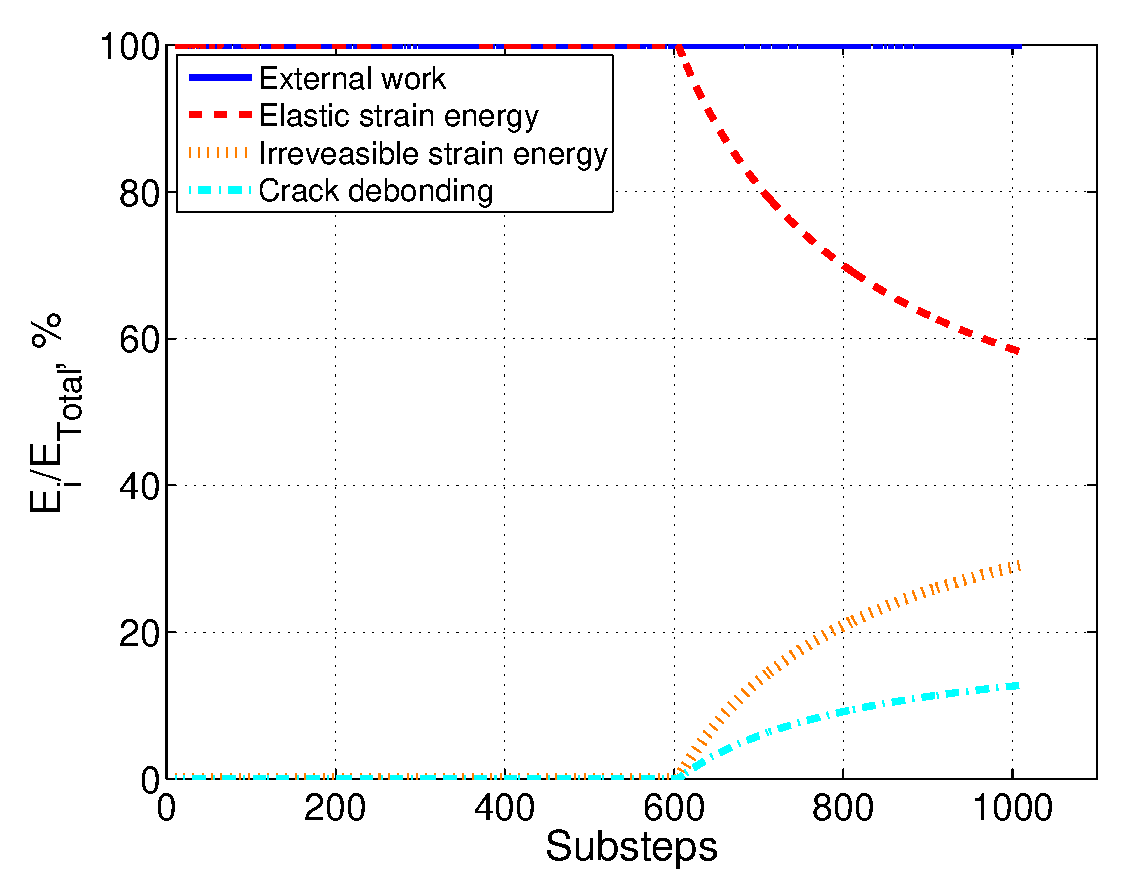
\includegraphics[width=\textwidth]{MRC/simple/tensile/energypercentage.eps}
\end{minipage}}
\caption{Energy in a uniaxial tensile test}
\label{fig:TensileEnergy}
\end{figure}

\item Shear test
\
\\
A pure shear test is simulated with $\sigma_{12}=60$ MPa pure shear stress.
\begin{figure}[htbp]
\subfigure[Types of Energy]{
\label{fig:TypesOfEnegyTen}
\begin{minipage}[b]{0.48\textwidth}
\centering
\vspace{-3cm}
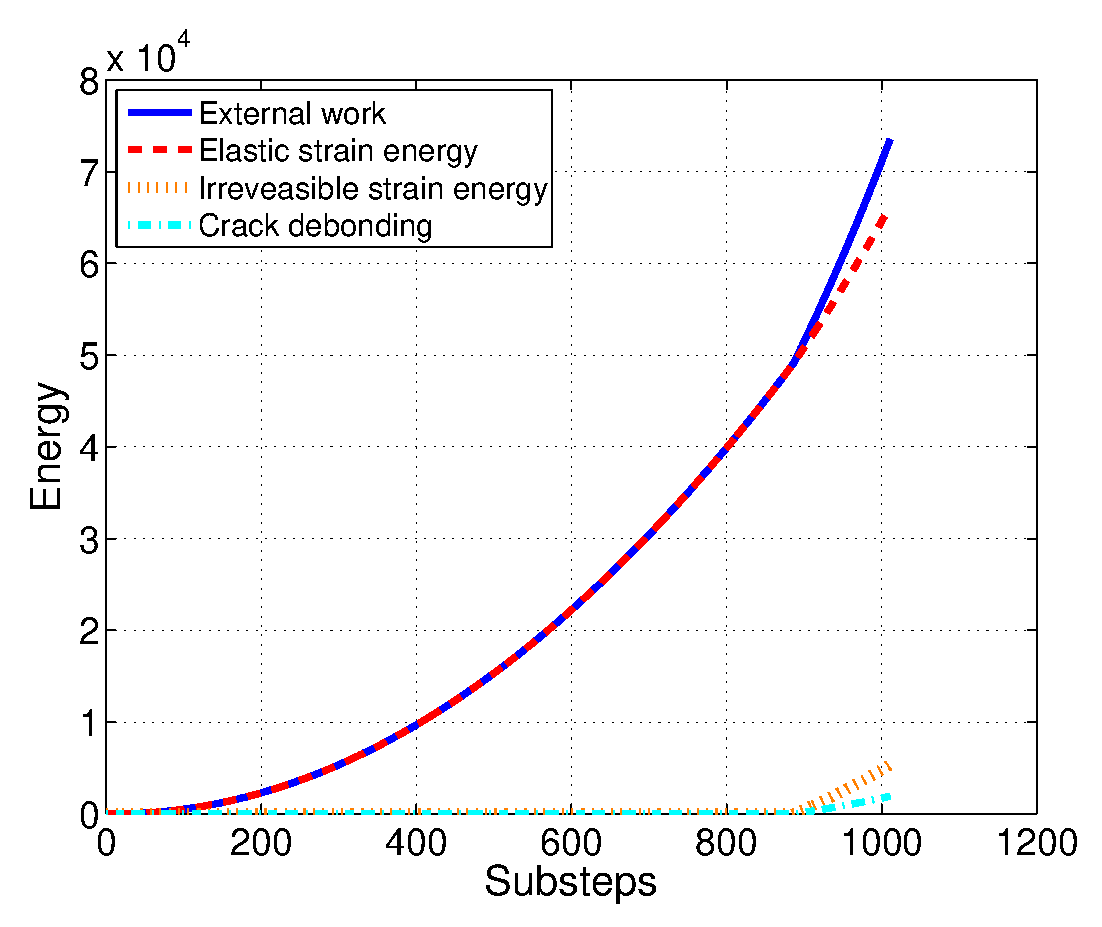
\includegraphics[width=\textwidth]{MRC/simple/shear/energy1.eps}
\end{minipage}}
\subfigure[Percentages of Each Energy]{
\label{fig:PercentagesOfEachEnergy}
\begin{minipage}[b]{0.48\textwidth}
\centering
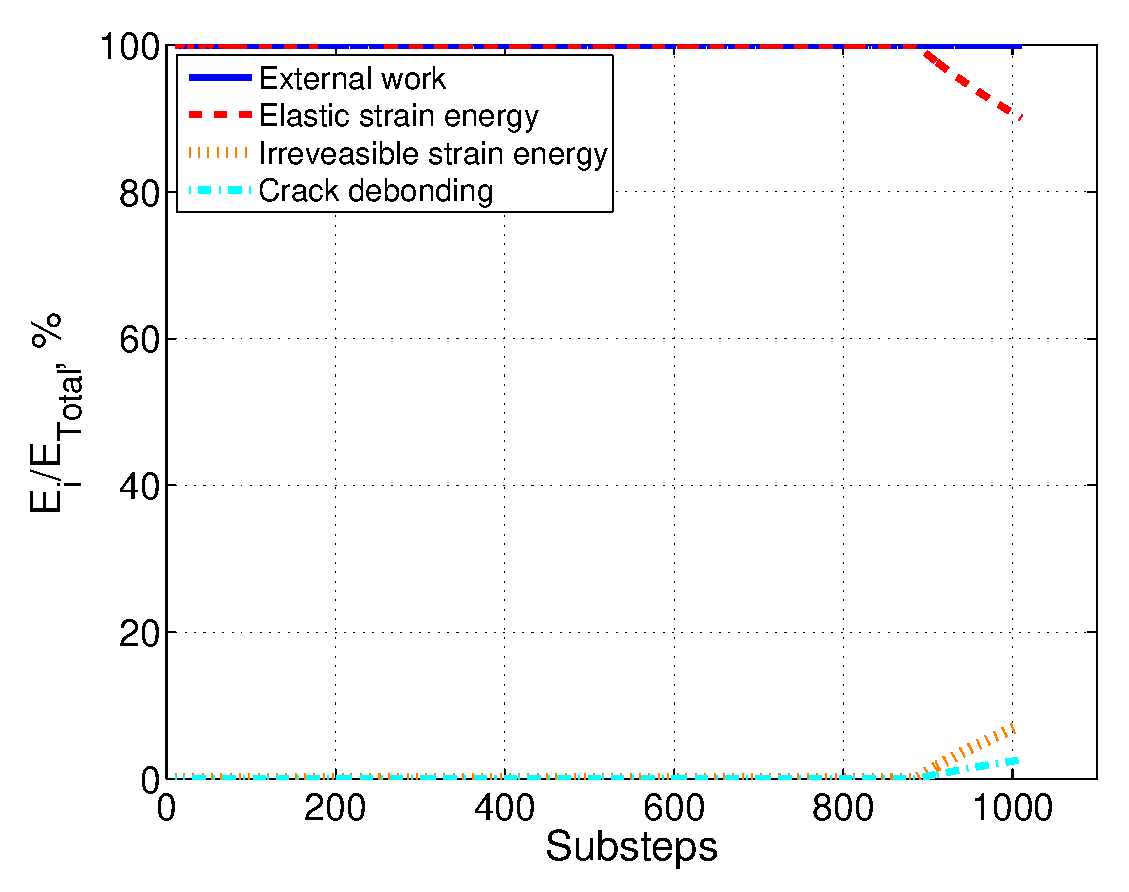
\includegraphics[width=\textwidth]{MRC/simple/shear/energypercentage.eps}
\end{minipage}}
\caption{Energy in a shear test}
\label{fig:ShearEnergy}
\end{figure}


\item Triaxial Compresion test
\
\\
A triaxial compression test is computed with a 30 MPa confining stress and a vertical 130 MPa compressive stress. Each energy term in this simulation is summarized as follows.
\begin{figure}[htbp]
\subfigure[Types of Energy]{
\label{fig:TypesOfEnegyTen}
\begin{minipage}[b]{0.48\textwidth}
\centering
\vspace{-3cm}
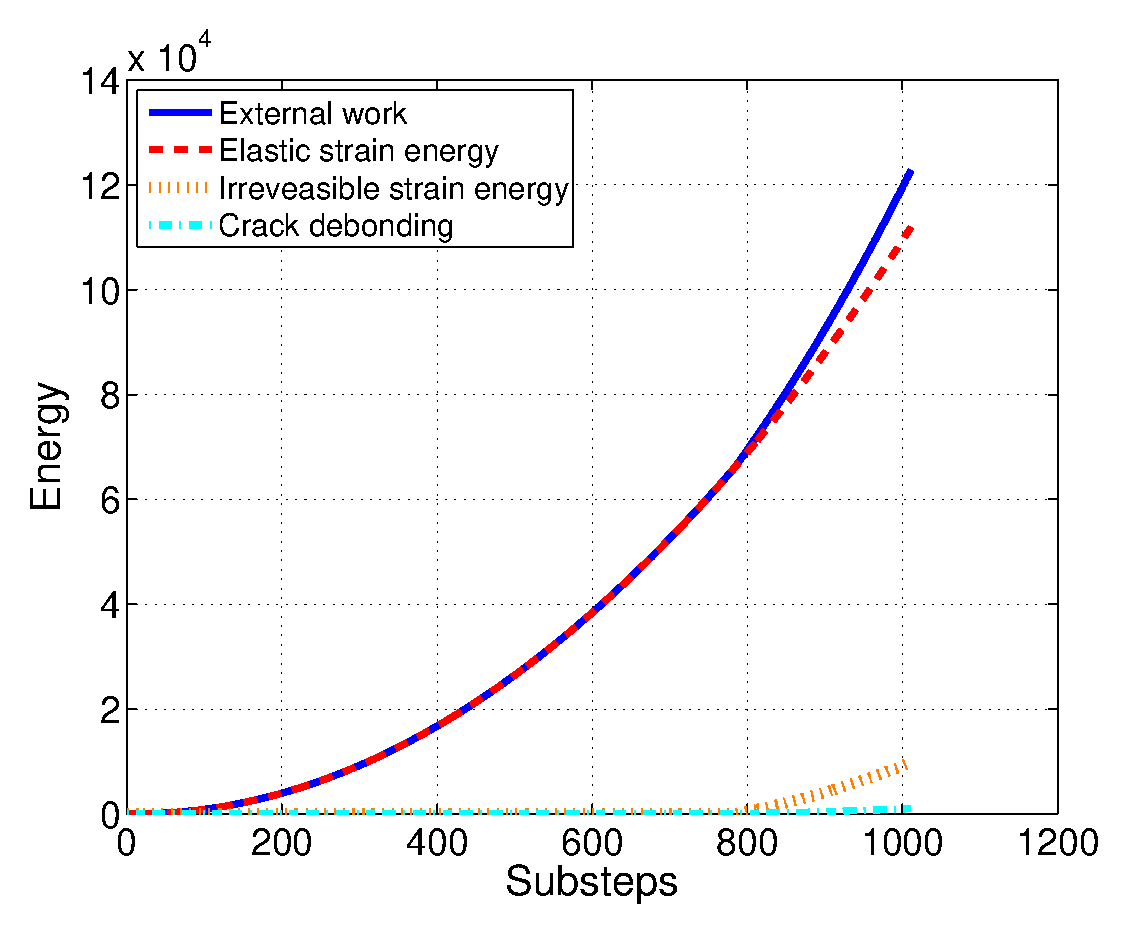
\includegraphics[width=\textwidth]{MRC/simple/compression/energy1.eps}
\end{minipage}}
\subfigure[Percentages of Each Energy]{
\label{fig:PercentagesOfEachEnergy}
\begin{minipage}[b]{0.48\textwidth}
\centering
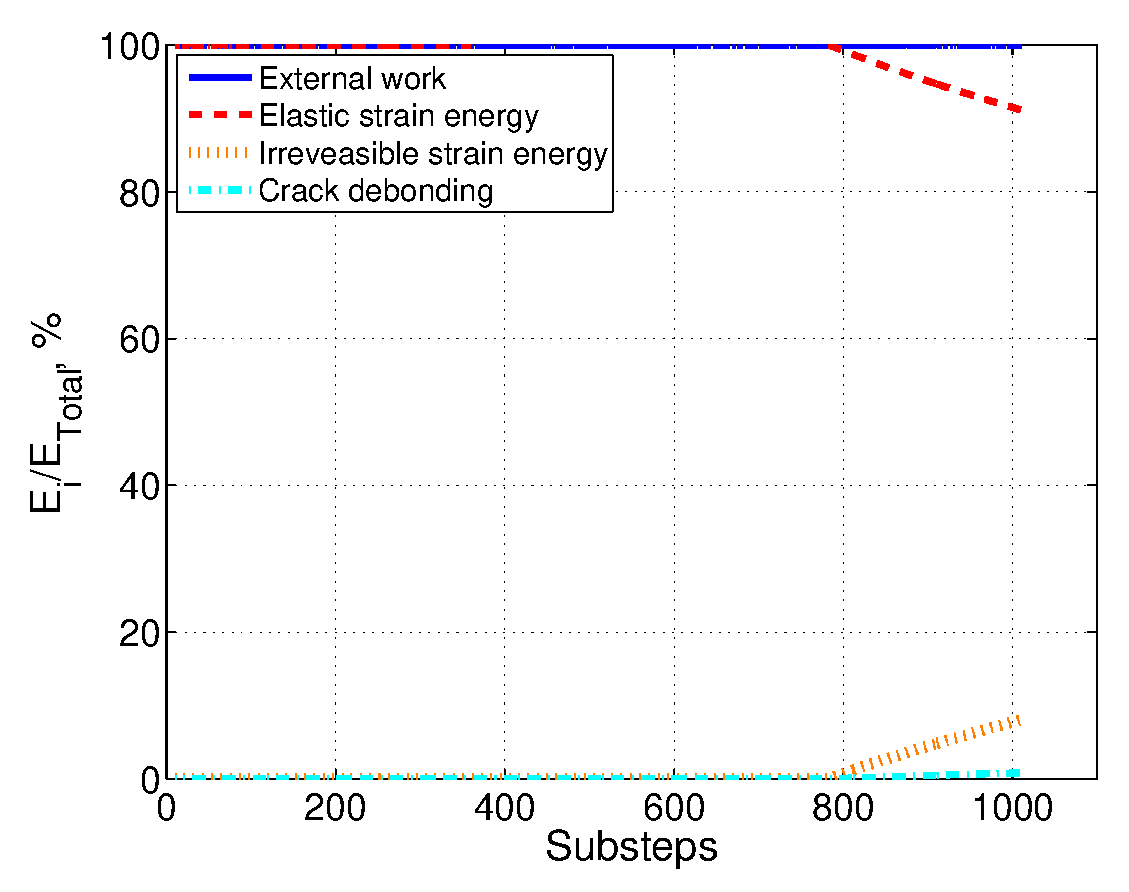
\includegraphics[width=\textwidth]{MRC/simple/compression/energypercentage.eps}
\end{minipage}}
\caption{Energy in a triaxial compression test}
\label{fig:CompressionEnergy}
\end{figure}
\end{enumerate}


\section{FEM simulation of damage dissipation driving propagation}
\subsection{Circular cavity}
\begin{enumerate}
\item intact rock mass
\item with initial CDM damage
\item with initial notch
\end{enumerate}

\begin{figure}[htbp]
   \centering
  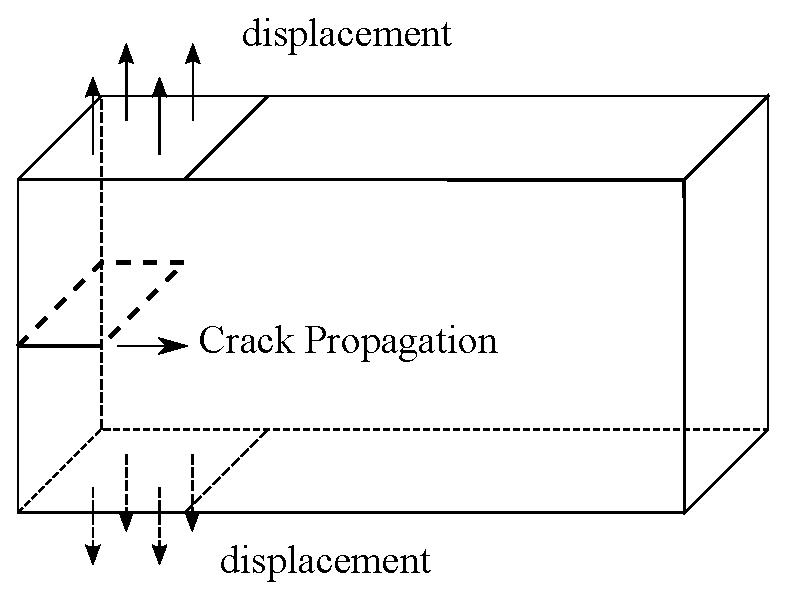
\includegraphics[width=0.6\textwidth]{inkscape/sketch/sketch.eps}
   \caption{Sketch of the simulation problem}
   \label{fig:sketch}
\end{figure}

The dissipated energy in XFEM is:
%
\begin{equation}
\label{eq:diss_XFEM}
    \int \dot\varPhi_{d} \, \ud t = \int G_c\dot{A} \,\ud{t}
\end{equation}

If the dissipated energy in different methods is equivalent, the relation between these methods can be obtained.
\begin{equation}
\label{eq:diss_XFEM}
    \int \bm\sigma:\dot{\bm\varepsilon}^{id}\,\ud{t}+\int\bm{Y}:\dot{\bm\varOmega}\,\ud{t} =
    \int G_c\dot{A} \,\ud{t}
\end{equation}
\subsection{with complex crack patterns}

% 
\subsection{Fracture patterns around cavities}


\section{Conclusion}



\section*{Acknowledgments}
This study was conducted at the Georgia Institute of Technology, as part of a research program on Finite Element Modeling of Hydraulic Fracturing. Funding was provided by ConocoPhillips, Houston, Texas.

%==================================================================
\appendix
\section{The DSID Model}

\subsection{Outline of the DSID Model}

For instance, \cite{Abualrub2010} and \cite{Cicekli2007} used a second-order damage tensor in a free energy potential expressed in terms of elastic strains, while \cite{Murakami1996} adopted the same approach with a different free energy expressed in terms of elastic strain and modified strains. However elastic strains cannot be controlled as such in an experiment of as a boundary condition in a numerical code. That is the reason why \cite{Halm1998} and \cite{Homand-Etienne1998} expressed rock skeleton free energy in terms of total strains. Their model turned out to be easier to calibrate against experimental data. \cite{Chaboche1993} and \cite{Pellet2005} employed a similar strategy, with the additional use of a parameter expressing the degree of anisotropy, allowing accounting for non-orthotropic damage. In uniaxial compression for instance, cracks can develop both parallel to the axis (orthotropic component of damage) and perpendicular to the axis (isotropic component of damage). An anisotropic damage model based on a stress-dependent free energy potential was proposed by \cite{Shao2005}; \cite{Shao2006}, \cite{Zhou2006} and \cite{Hayakawa1997}. \cite{Hayakawa1997} used a modified stress tensor to account for the difference between compressive and tensile stress. The damage evolution law derives from a criterion expressed in terms of the energy release rate conjugate to damage. In the former models on the contrary, damage evolution law is not derived from the damage potential with the energy release rate that is conjugate to damage: damage rate is calculated using associated variables used to predict crack lengths. Differences between the afore-mentioned damage models are highlighted in Table \ref{aniso_models}.

\begin{sidewaystable}
\resizebox{\textheight}{!}{
\setlength\tabcolsep{2pt}
\begin{tabular}{p{1.5cm}|l@{}|p{3.5cm}|l|p{2.3cm}|p{2cm}}
\hline
     Models
  & \multicolumn{1}{|c|}{Free energy}
  & \scriptsize{Damage criterion or damage evolution law}
  & \footnotesize{Driving force}
  & \footnotesize{Stress Variables}
  & \footnotesize{Strain Variabless}
\\  \hline
    {\scriptsize \cite{Abualrub2010,Cicekli2007}}
  &  \multicolumn{1}{|l|}{ \footnotesize{$\psi_s(\bm\varepsilon^e,\bm\phi^{\pm},\varepsilon^{\pm}_{eq},\phi^{\pm}_{eq})$} }
  &   \footnotesize{$f_d^{\pm}(\bm{Y}^{\pm},\phi_{eq}^{\pm})$}
  &   \footnotesize{$\bm{Y}^{\pm}$}
  &  \footnotesize{$\bm\sigma^{\pm}$}
  &   \footnotesize{$\bm\varepsilon^{e}$ and $\bm\varepsilon_{eq}$}
\\
  &  \footnotesize{$=\psi^e(\bm\varepsilon^e,\bm\phi^{\pm})+\Psi^p(\varepsilon^{\pm}_{eq})+\psi^d(\phi^{\pm}_{eq})$}
  & & & &
\\[2mm] \hline
     {\scriptsize\cite{Murakami1996}}
  &  \multicolumn{1}{|l|}{\footnotesize{$\psi_s=\psi^e(\bm\varepsilon^e,\bm\varOmega)+\psi^d(\beta)$}}
  &  \footnotesize{$f_d(\bm{Y},\beta)$}
  &  \footnotesize{$\bm{Y}$}
  &
  &  \footnotesize{$\bm\varepsilon^e$ and $\bar{\bm\varepsilon}^e$}
\\ [2mm]
\hline
     {\scriptsize\cite{Halm1998,Homand-Etienne1998}}
  &  \footnotesize{$\psi_s(\bm\varepsilon,\bm\varOmega)$}
  &  \footnotesize{$f_d(\bm{Y}^+,\bm\varOmega)$}
  &  \footnotesize{$\bm{Y}^{+}=g\bm\varepsilon^+$}
  &
  &  \footnotesize{$\bm\varepsilon$ and $\bm\varepsilon^{\pm}$}
\\
[2mm] \hline
     {\scriptsize\cite{Chaboche1993}}
  &  \footnotesize{$\psi_s(\bm\varepsilon,d_i)$}
  &  \footnotesize{$\bm{Q}^*=(1-\xi)\bm{I}+\xi\bm\Gamma^*$}
  &  \footnotesize{$\bm{Y}$}
  &
  &  \footnotesize{$\bm\varepsilon$}
\\
  &
  &  \footnotesize{$\dot{\bm\varOmega}=\dot{\mu}\mathbb{Q}^*$}
  & & &
\\
[2mm] \hline
     {\scriptsize\cite{Pellet2005}}
  &  \footnotesize{$\psi_s(\bm\varepsilon^e,p,\bm\varOmega)$}
  &  \footnotesize{$\dot{\bm\varOmega}=\mathbb{S}:\bm{Y}$}
  &  \footnotesize{$\bm{Y}$}
  &  \footnotesize{$\bm\sigma$ and effective}
  &  \footnotesize{$\bm\varepsilon^e$}
\\
  &
  &  \footnotesize{$\mathbb{S}=(\beta-1)\mathbb{I}+\bm{I}\otimes\bm{I}$}
  &
  &  \footnotesize{stress $\hat{\bm\sigma}$}
  &
\\
[2mm] \hline
     {\scriptsize\cite{Shao2005,Shao2006,Zhou2006}}
  &  \footnotesize{$\psi_s(\bm\sigma,\bm\varOmega)$}
  &  \footnotesize{based on micro-}
  &  \footnotesize{not included}
  &  &
\\
  &
  &  \footnotesize{mechanics concepts}
  & & &
\\
[2mm] \hline
     {\scriptsize\cite{Hayakawa1997}}
  &  \footnotesize{$\psi_s(\bm\sigma,r,\bm\varOmega,\beta)$}
  &  \footnotesize{$f_d(\bm{Y},r,\bm\varOmega)$}
  &  \footnotesize{$\bm{Y}$}
  &  \footnotesize{$\bm\sigma$ and $\bar{\bm\sigma}$}
  &
\\
[2mm] \hline
\end{tabular}}%
\caption{Comparison of Several Model Formulations for Anisotropic Damage.}
\label{aniso_models}%
\end{sidewaystable}

Most anisotropic damage models for geomaterials postulate a skeleton free energy expressed in terms of deformation. As a result, the energy release rate \textbf{Y} (also called damage driving force) conjugate to damage  is also a function of deformation. In order to capture cracks due to ``splitting effects'' (i.e. Griffith cracks) and equivalent cracks due to ``crossing effects'' (i.e. wing shear cracks), it is necessary to make the damage criterion depend on a tensile damage driving force. In order to better account for states of tensile deformation under differential stress, the proposed anisotropic damage model is hyper-elastic, and a free energy potential expressed as a term of stress (Gibbs free energy, $G_s$) is proposed. This free energy accounts for the surface energy dissipated by opened cracks and closed cracks, and the elastic energy stored in material as well. To stay within the framework of linear elasticity in the absence of damage, the expression of the free energy should have at most quadratic terms of $\bm\sigma$ \cite{Halm1998, Shao2005}
. The thermodynamic framework of the DSID model is summarized in Table.~\ref{tab:DSID}. Stress/strain relationships are derived from the expression of a free energy potential. Damage evolution is controlled by a damage function, similar to Drucker-Prager yield function (but depending on the energy release rate). The damage flow rule is non-associate, and the damage potential is chosen so as to ensure the positivity of dissipation associated to damage. The irreversible deformation due to damage follows an associated flow rule, which allows representing physical anisotropic trends of the deformation tensor during the damage process. More details are provided in \cite{Xu2014}.
\
\begin{table}
\caption{Thermodynamic framework of the DSID model} \label{tab:DSID}
\small{
\begin{center}
{
\renewcommand{\arraystretch}{1.05}
\begin{tabular}{p{5cm}p{5cm}p{5cm}}
\hline
     \multicolumn{3}{c}{\textbf{D.S.I.D. Model}}
\\ [1mm] \hline %[2mm]
     \multicolumn{1}{l}{\footnotesize{\textbf{Free Energy}} }
  & \multicolumn{2}{l}{ \footnotesize{$G_s(\bm\sigma, \bm\varOmega)=\dfrac{1}{2}\bm\sigma:\mathbb{S}_0:\bm\sigma+a_1\,\textrm{Tr}
     \bm\varOmega(\textrm{Tr}\bm\sigma)^2+a_2\,\textrm{Tr}(\bm\sigma\cdot\bm\sigma\cdot\bm\varOmega)$} }
\\ 
      \multicolumn{1}{c}{ }
  &  \multicolumn{2}{c}{ \footnotesize{$+a_3\,\textrm{Tr}\bm\sigma
      \,\textrm{Tr}(\bm\varOmega\cdot\bm\sigma)+a_4\,\textrm{Tr}\bm\varOmega\,\textrm{Tr}(\bm\sigma\cdot\bm\sigma)$}}
\\ 
     \multicolumn{1}{l}{}
  & \multicolumn{2}{l}{ \footnotesize{$\bm\varepsilon^E = \dfrac{\partial G_s}{\partial \bm\sigma}
   = \dfrac{1+\nu_0}{E_0}\bm\sigma-\dfrac{\nu_0}{E_0}(\textrm{Tr}\bm\sigma)\,\bm\delta
   + 2a_1(\textrm{Tr}\bm\varOmega\,\textrm{Tr}{\bm\sigma})\,\bm\delta+a_2(\bm\sigma\cdot\bm\varOmega+\bm\varOmega\cdot\bm\sigma)
    $}}
\\ 
     \multicolumn{1}{c}{ }
  &  \multicolumn{2}{c}{ \footnotesize{$+ a_3[\,\textrm{Tr}(\bm\sigma\cdot\bm\varOmega)\,\bm\delta+(\textrm{Tr}\bm\sigma)\,\bm\varOmega \, ]
    + 2a_4(\textrm{Tr}\bm\varOmega)\,\bm\sigma$}}
\\ 
     \multicolumn{1}{c}{ }
  &  \multicolumn{2}{l}{ \footnotesize{$ \bm{Y}  = \dfrac{\partial G_s}{\partial \bm
      \varOmega} =   a_1(\textrm{Tr}\bm\sigma)^2\,\bm\delta + a_2\bm\sigma \cdot \bm\sigma + a_3\textrm{Tr}(\bm\sigma)\bm\sigma +a_4\textrm{Tr}(\bm\sigma
    \cdot \bm\sigma)\bm\delta$}}
\\  [1mm] \hline
       \multicolumn{1}{l}{\footnotesize{\textbf{Damage Function}} }
  &   \multicolumn{2}{l}{ \footnotesize{$f_d=\sqrt{J^*}-\alpha I^*-k $}}
\\ 
     \multicolumn{1}{l}{}
  &   \multicolumn{2}{l}{ \footnotesize{$J^*= \dfrac{1}{2}(\mathbb{P}_1:\bm{Y}-\frac{1}{3}I^*\bm\delta):(\mathbb{P}_1:\bm{Y}
     -\frac{1}{3}I^*\bm\delta), \quad I^*= \left(\mathbb{P}_1:\bm{Y}\right):\bm\delta$}}
\\ 
      \multicolumn{1}{c}{ }
  &   \multicolumn{2}{l}{ \footnotesize{$\mathbb{P}_1\left(\bm{\sigma}\right)=\sum_{p=1}^{3}\left[H(\sigma^{(p)})-H(-\,\sigma^{(p)})\right]
      \bm{n}^{(p)}\otimes\bm{n}^{(p)}\otimes\bm{n}^{(p)}\otimes\bm{n}^{(p)}$}}
\\ 
      \multicolumn{1}{c}{ }
  &   \multicolumn{2}{l}{\footnotesize{$k=C_0-C_1\textrm{Tr}(\bm\varOmega)$}}
\\ [1mm] \hline
     \multicolumn{1}{l}{\footnotesize{\textbf{Damage Potential}}}
  & \multicolumn{2}{l}{\footnotesize{$g_d = \sqrt{\dfrac{1}{2}(\mathbb{P}_2:\bm{Y}):(\mathbb{P}_2:\bm{Y})}$}}
\\ 
      \multicolumn{1}{c}{ }
  &   \multicolumn{2}{l}{\footnotesize{$\mathbb{P}_2=\sum_{p=1}^{3}H\left[\max_{q=1}^{3}(\sigma^{(q)})-\sigma^{(p)}\right]\,
     \bm{n}^{(p)}\otimes\bm{n}^{(p)}\otimes\bm{n}^{(p)}\otimes\bm{n}^{(p)}$}}
\\ [1mm] \hline
     \multicolumn{1}{l}{\footnotesize{\textbf{Flow Rule} }}
  &   \multicolumn{2}{l}{\footnotesize{$\dot{\bm\varepsilon}^{id}  = \dot{\lambda}_d \dfrac{\partial f_d}{\partial \bm\sigma} =
       \dot{\lambda}_d \dfrac{\partial f_d}{\partial \bm{Y}}:\dfrac{\partial \bm{Y}}{\partial \bm\sigma}$}}
\\ 
      \multicolumn{1}{c}{ }
  &   \multicolumn{2}{l}{\footnotesize{$\dot{\bm\varOmega}  = \dot{\lambda}_d \dfrac{\partial g_d}{\partial \bm{Y}}$}}
\\ [1mm] \hline
      \multicolumn{1}{p{5cm}}{$G_s$: Gibbs free energy }
  &  \multicolumn{1}{p{5cm}}{$\bm\sigma$: Stress tensor}
  &  \multicolumn{1}{p{5cm}}{$\bm\varOmega$: Damage variable}
\\ 
      \multicolumn{1}{p{5cm}}{$\bm\varepsilon^E$: Total elastic strain}
  &  \multicolumn{1}{p{5cm}}{$\nu_0$: Poisson's ratio}
  &  \multicolumn{1}{p{5.7cm}}{$\mathbb{S}_0$: Undamaged compliance tensor}
\\ 
      \multicolumn{1}{p{5cm}}{$E_0$: Young's Modulus}
  &  \multicolumn{1}{p{5cm}}{$\bm\delta$: Kronecker delta}
  &  \multicolumn{1}{p{5cm}}{$\bm{Y}$: Damage driving force}
\\ 
      \multicolumn{1}{p{5cm}}{$f_d$: Damage function}
  &  \multicolumn{1}{p{5cm}}{$\mathbb{P}_1$ and $\mathbb{P}_2$: Projection tensors}
  &  \multicolumn{1}{p{5cm}}{$H(\cdot)$: Heaviside function}
\\ 
      \multicolumn{1}{p{5cm}}{$C_0$: Initial damage threshold}
  &  \multicolumn{1}{p{5cm}}{$g_d$: Damage potential}
  &  \multicolumn{1}{p{5cm}}{$\textrm{max}(\cdot)$: Maximum function}
\\ 
      \multicolumn{1}{p{5cm}}{$\dot{\bm\varepsilon}^{id}$: Irreavisible strain rate}
  &  \multicolumn{1}{p{5cm}}{$\dot\lambda_d$: Lagrangian Multiplier}
  &  \multicolumn{1}{p{5cm}}{$\dot{\bm\varOmega}$: Damage rate}
\\ 
      \multicolumn{1}{p{4.3cm}}{$a_1$, $a_2$, $a_3$, $a_4$: Material parameters}
  &  \multicolumn{1}{p{5cm}}{$\sigma^{(p)}$ and $\bm{n}^{(p)}$: Principal stress and corresponding direction}
  &  \multicolumn{1}{p{5.3cm}}{$C_1$: Damage hardening variable}
\\ [1mm] \hline
\end{tabular}
}
\end{center}
}
\end{table}


%% The Appendices part is started with the command \appendix;
%% appendix sections are then done as normal sections
%% \appendix

%% \section{}
%% \label{}

%% References
%%
%% Following citation commands can be used in the body text:
%% Usage of \cite is as follows:
%%   \cite{key}          ==>>  [#]
%%   \cite[chap. 2]{key} ==>>  [#, chap. 2]
%%   \citet{key}         ==>>  Author [#]

%% References with bibTeX database:

\bibliographystyle{model1a-num-names}
\bibliography{biblio}

%% Authors are advised to submit their bibtex database files. They are
%% requested to list a bibtex style file in the manuscript if they do
%% not want to use model1a-num-names.bst.

%% References without bibTeX database:

% \begin{thebibliography}{00}

%% \bibitem must have the following form:
%%   \bibitem{key}...
%%

% \bibitem{}

% \end{thebibliography}

%%==========================================================================================

\end{document}
%%
%% End of file `elsarticle-template-1a-num.tex'.
